\documentclass{beamer}

\usepackage[utf8]{inputenc}
\usepackage{amsmath}
\usepackage{graphicx}
\usepackage{pdflscape}
\usepackage{geometry}

\setbeamertemplate{caption}[numbered]

\title{Neural mechanisms in processing of emotion in real and virtual faces}
\subtitle{A functional near-infrared spectroscopy (fNIRS) study}
\author{Dylan Rapanan}
\date{\today}

\begin{document}

\begin{frame}
    \titlepage
\end{frame}

% display C:\Users\super\OneDrive - Ontario Tech University\fNIRS_Emotions\plots\figures\Paradigm.png
\begin{frame}
    \frametitle{Task Paradigm}
    \begin{figure}
        \centering
        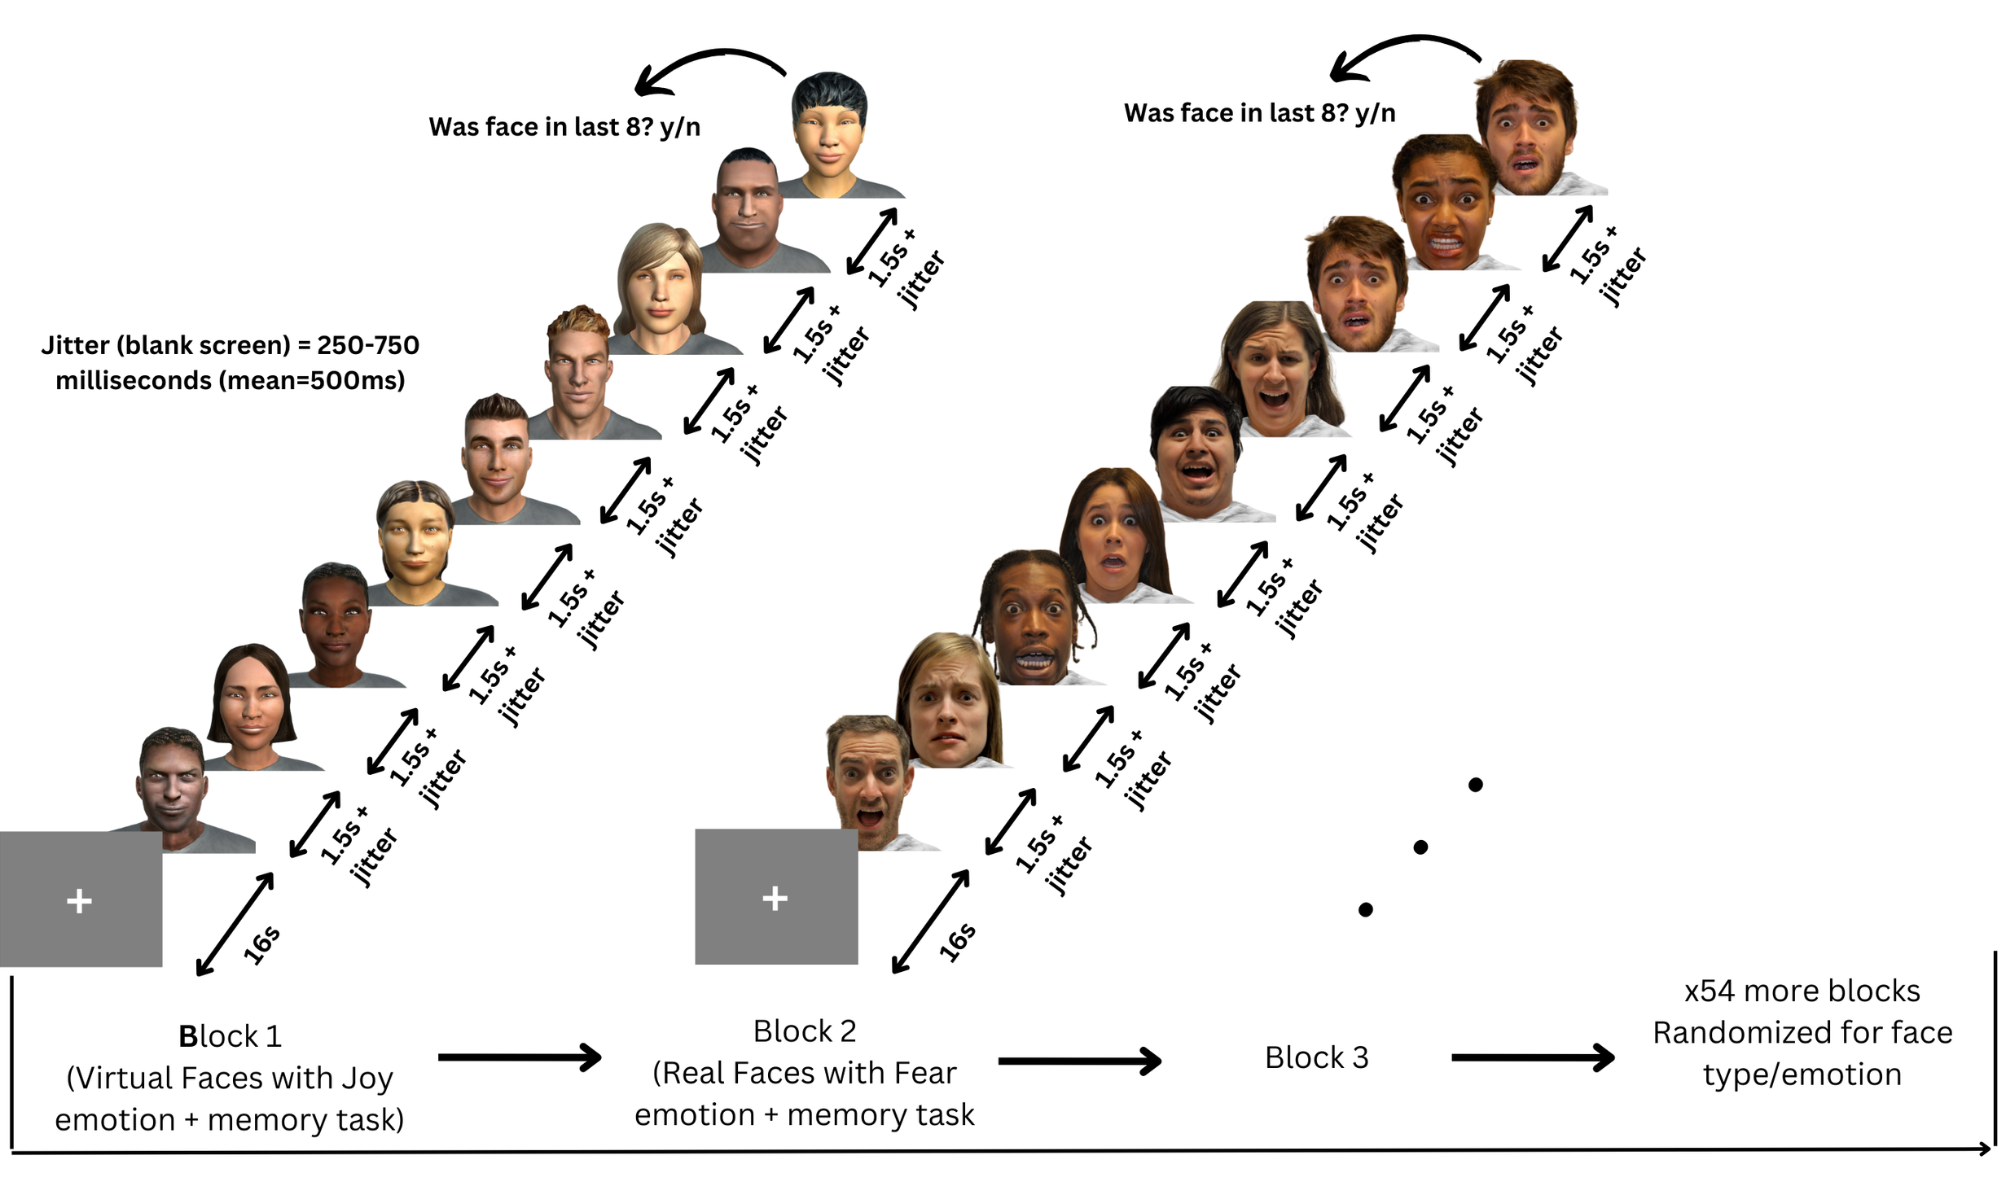
\includegraphics[width=0.8\textwidth]{C:/Users/super/OneDrive - Ontario Tech University/fNIRS_Emotions/plots/figures/Paradigm.png}
        \caption{Participants viewed 56 blocks of 8 faces (4 male, 4 female) from two sets:
        real (RADIATE) and virtual (UIBVFED). Each face displayed one of 7
        emotions (anger, disgust, fear, happiness, sadness, surprise, neutral)}
    \end{figure}
\end{frame}

% display C:\Users\super\OneDrive - Ontario Tech University\fNIRS_Emotions\plots\figures\Montage.png
\begin{frame}
    \frametitle{fNIRS Montage}
    \begin{minipage}[t]{0.55\textwidth}
        \vspace{-\baselineskip}
        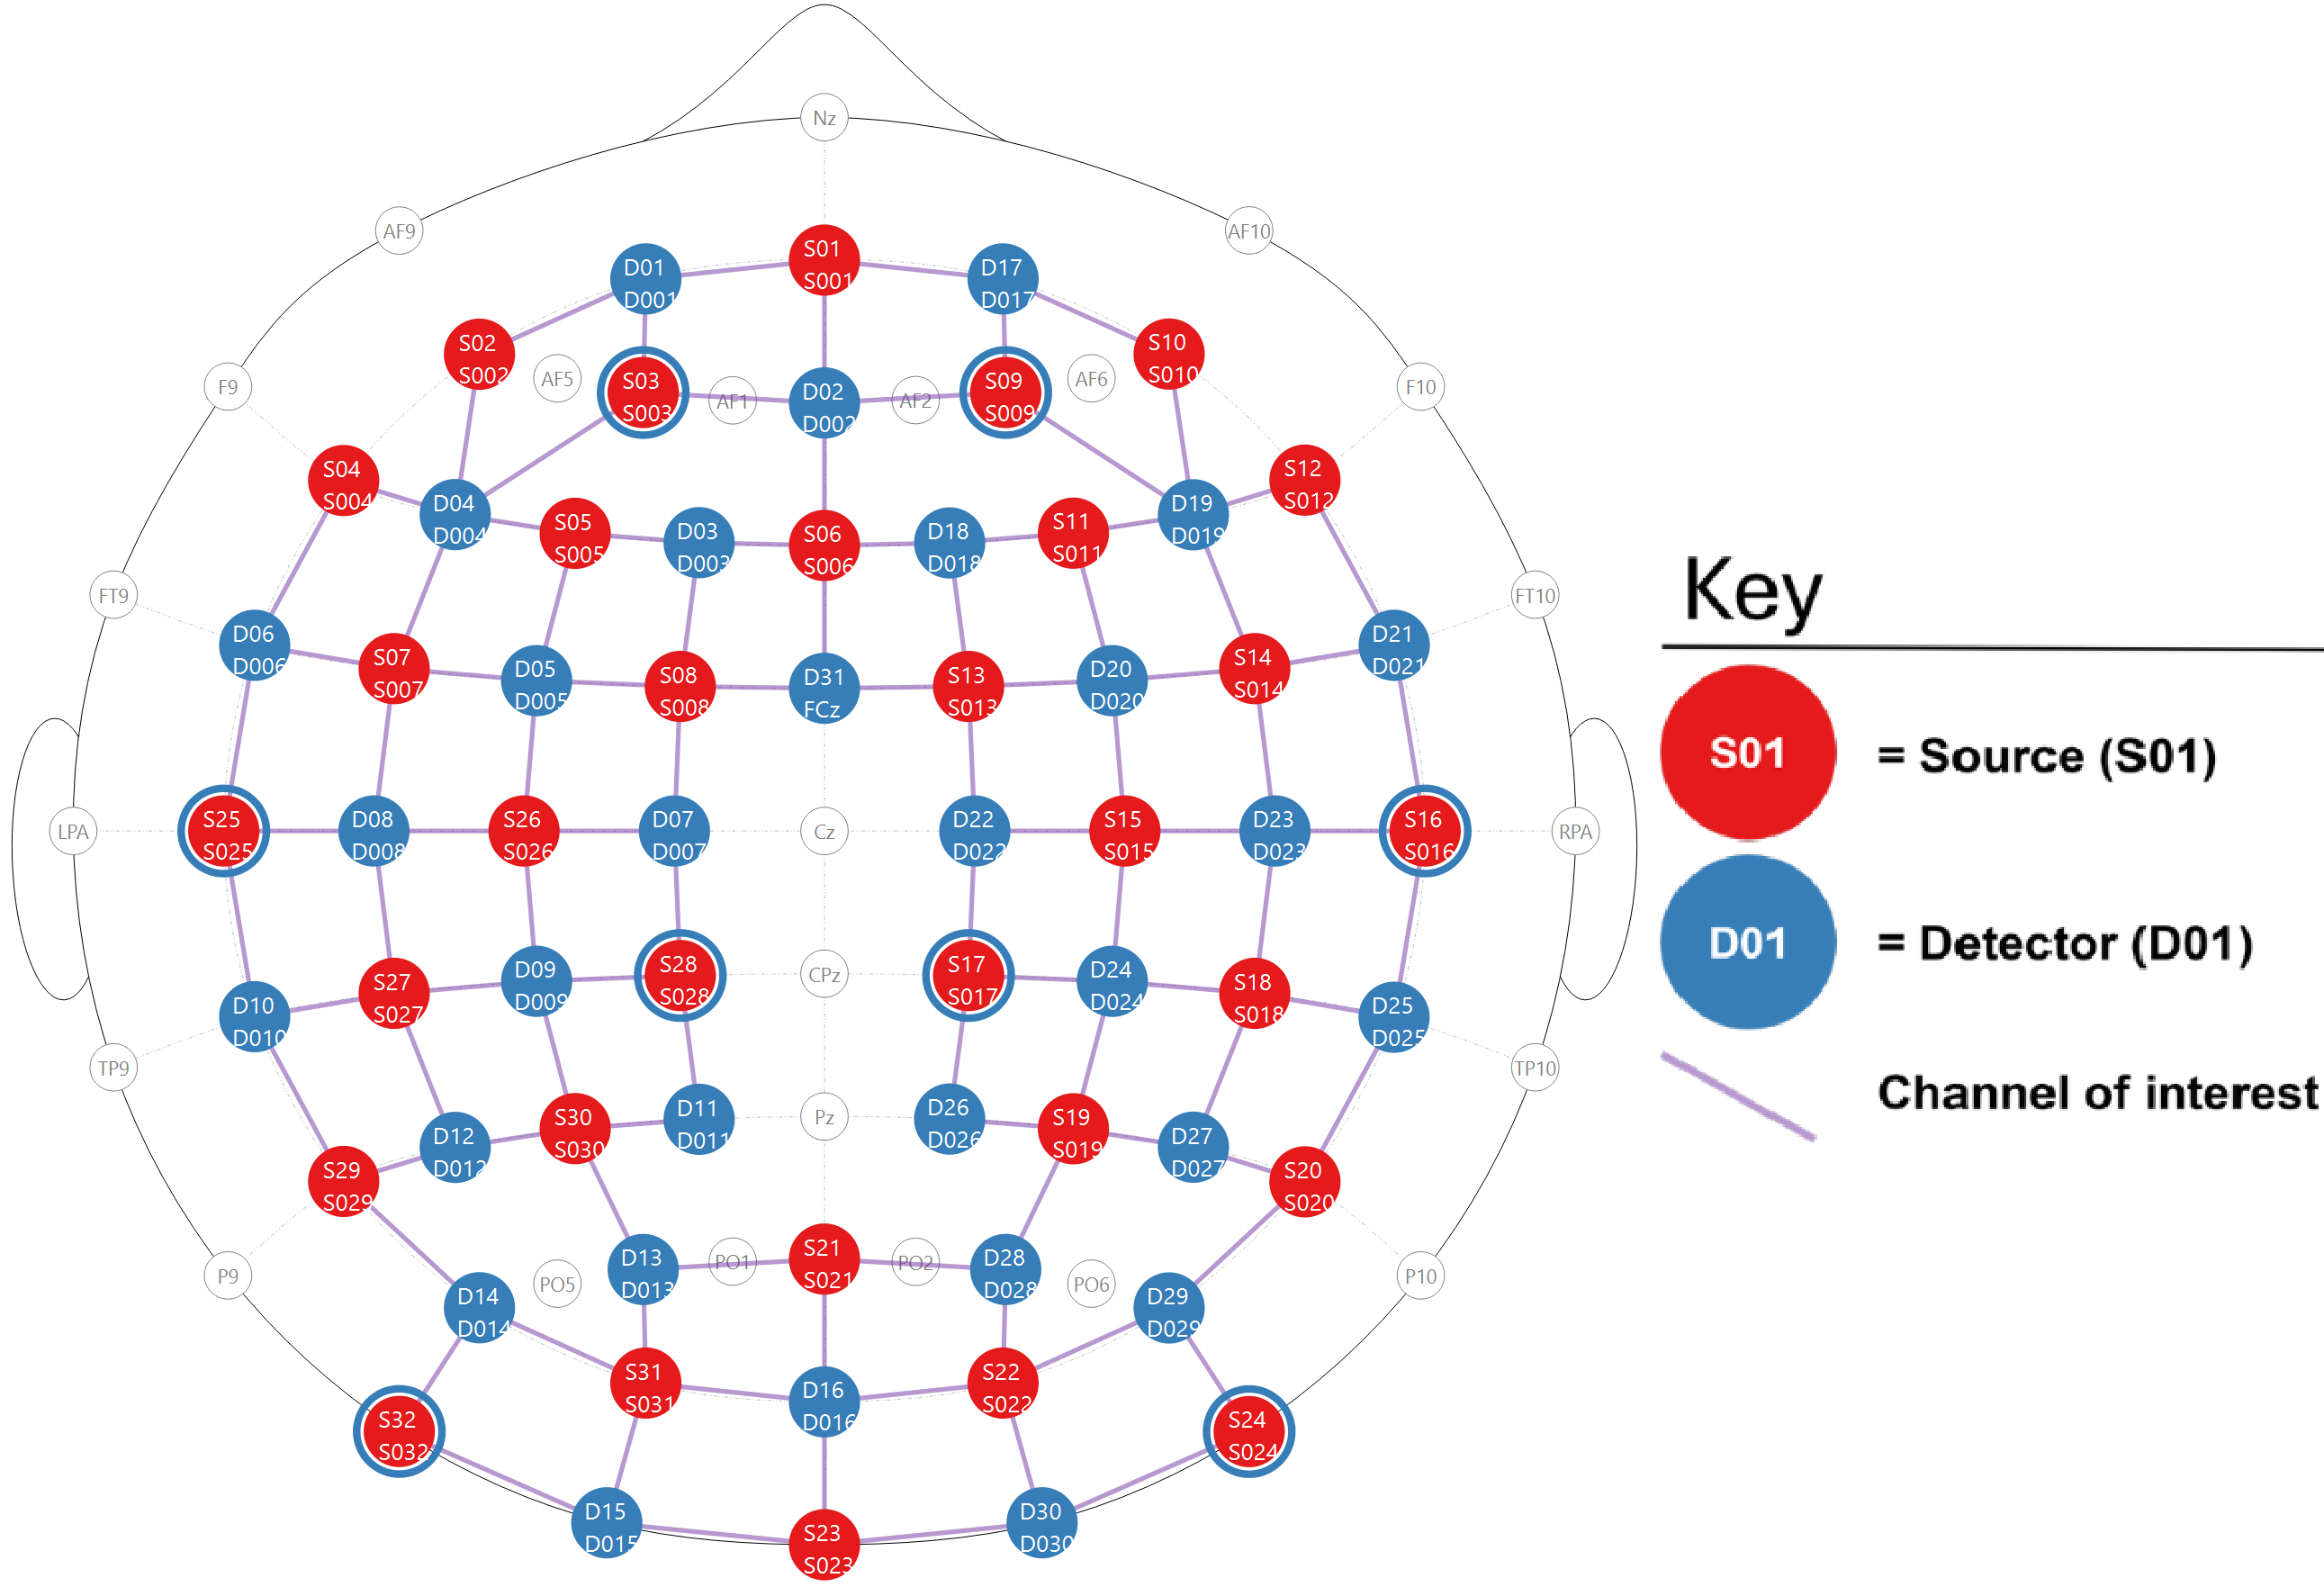
\includegraphics[width=\textwidth]{C:/Users/super/OneDrive - Ontario Tech University/fNIRS_Emotions/plots/figures/Montage.png}
    \end{minipage}
    % display C:\Users\super\OneDrive - Ontario Tech University\fNIRS_Emotions\plots\figures\Montage legend.png next to the above image
    \begin{minipage}[t]{0.2\textwidth}
        \vspace{-\baselineskip}
        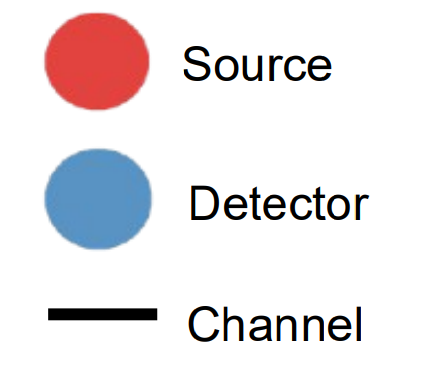
\includegraphics[width=\textwidth]{C:/Users/super/OneDrive - Ontario Tech University/fNIRS_Emotions/plots/figures/Montage legend.png}
    \end{minipage}
    \begin{figure}
        \caption{High density 32x32 fNIRS probe layout with 206 channels. \newline
        fNIRS data recorded using two NIRSport2 systems with sampling rate: 6.105 Hz at wavelengths: 760 $nm$ and 850 $nm$.}
    \end{figure}
\end{frame}

% display C:\Users\super\OneDrive - Ontario Tech University\fNIRS_Emotions\plots\signal quality\Percentage of Good Windows.png
\begin{frame}
    \frametitle{Signal Quality}
    \begin{figure}
        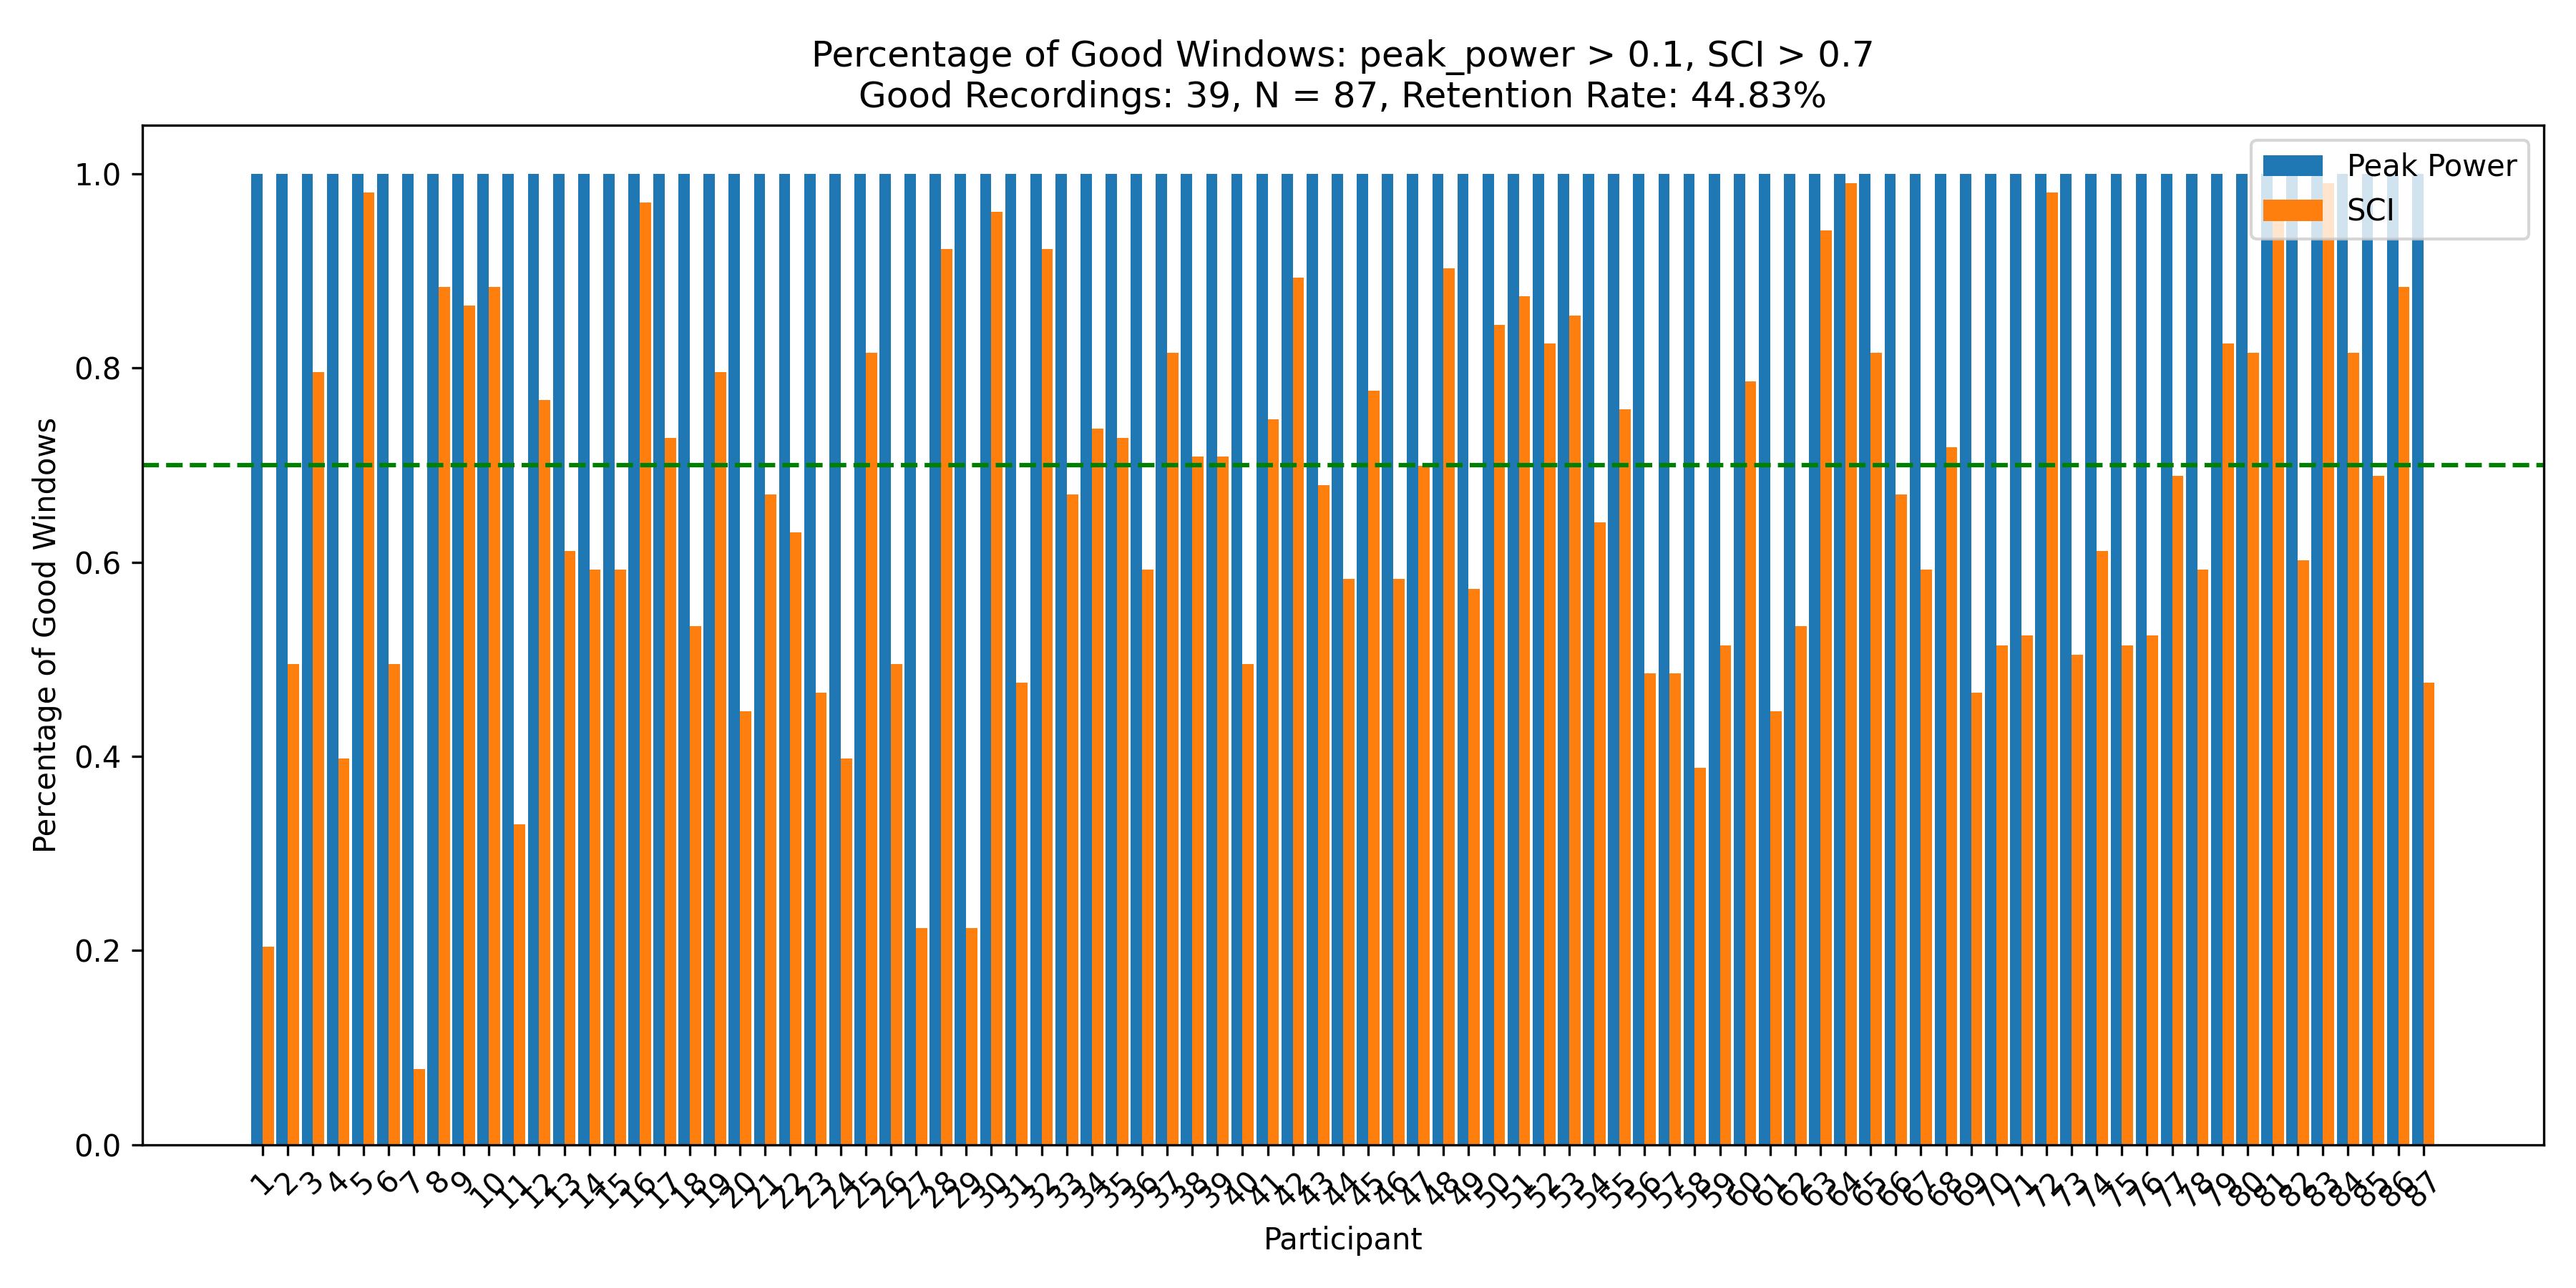
\includegraphics[width=1\textwidth]{C:/Users/super/OneDrive - Ontario Tech University/fNIRS_Emotions/plots/signal quality/Percentage of Good Windows.png}
        \caption{Peak power $<$ 0.1 and the Scalp Coupling Index (SCI) $<$ 0.7 were calculated for 5s sliding windows for each channel for each participant.
        The dotted green line represents the 70\% threshold for good windows.
        }
            \begin{itemize}
                \item If $>$ 70\% of the windows in a channel were good, the channel was deemed good.
                \item If $>$ 70\% of the channels in a participant were good, the participant was deemed good.
                \item Out of 87 participants, 39 are currently deemed good.
            \end{itemize}
    \end{figure}
\end{frame}

% display C:\Users\super\OneDrive - Ontario Tech University\fNIRS_Emotions\plots\signal quality\Average SCI (Windowed) per Channel\All Participants.png
\begin{frame}
    \frametitle{Signal Quality by Channel}
    \begin{figure}
        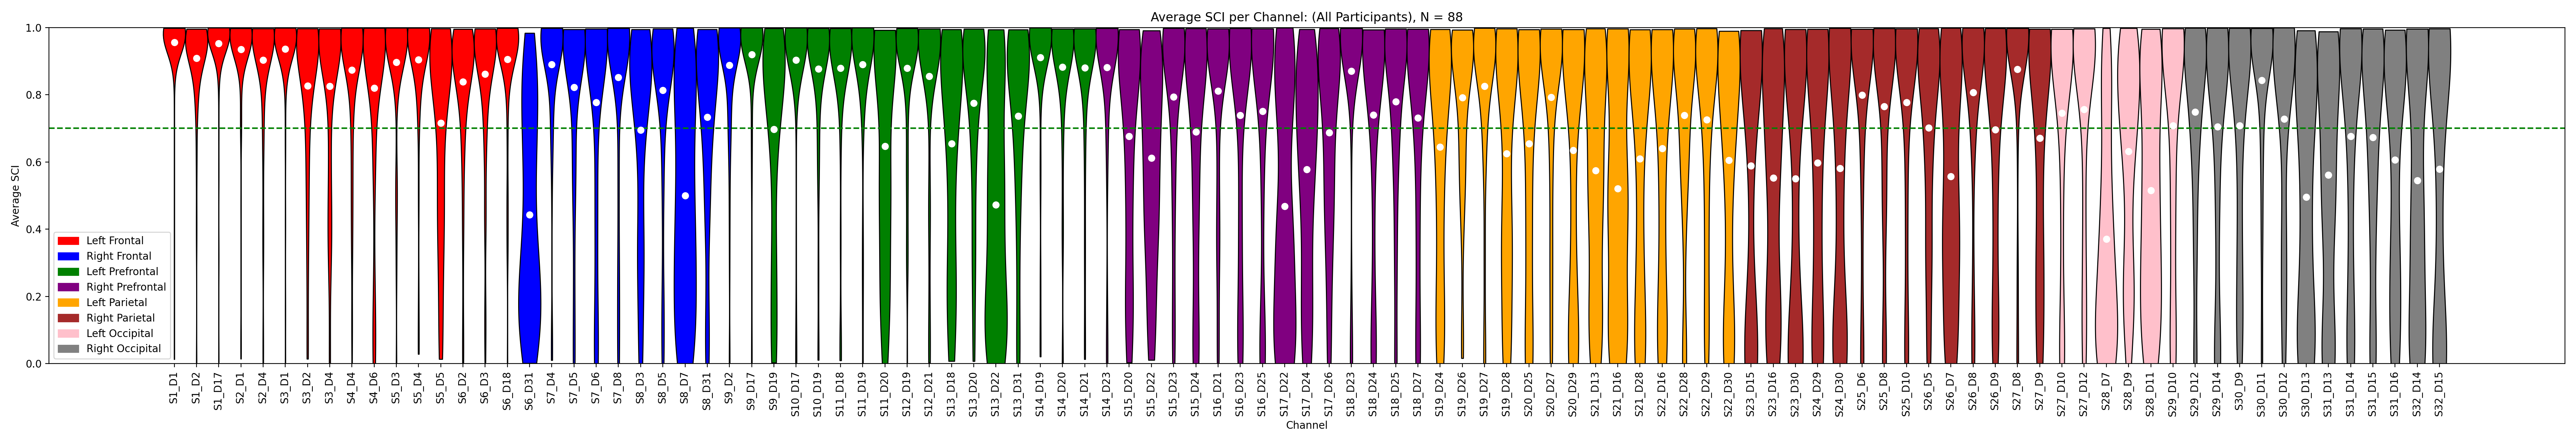
\includegraphics[width=1\textwidth]{C:/Users/super/OneDrive - Ontario Tech University/fNIRS_Emotions/plots/signal quality/Average SCI (Windowed) per Channel/All Participants.png}
        \caption{Average SCI for each channel across all participants. The channels are color coded by brain region. The wider the line, the more participants had a SCI value in that range.}
            \begin{itemize}
                \item We can see that the channels towards the back of the head tend to have lower SCI values (this may be because people have lots of hair at the back of their head).
                \item There are a select few channels that have low SCI values across all participants. 
            \end{itemize}
    \end{figure}
\end{frame}

% display C:\Users\super\OneDrive - Ontario Tech University\fNIRS_Emotions\plots\figures\Sample Design Matrix.png
\begin{frame}{General Linear Model (GLM) Analysis}
    \begin{itemize}
      \item \textbf{Design Matrix Construction:}
        \begin{itemize}
          \item Use a cosine drift model with high-pass filtering (cutoff = 0.03125 Hz; $\sim$32\,s period) to remove low-frequency trends.
          \item Model the haemodynamic response with the Statistical Parametric Mapping (SPM) Haemodynamic Response Function (HRF) over a 16s stimulus duration.
        \end{itemize}
    \end{itemize}
    \begin{figure}
        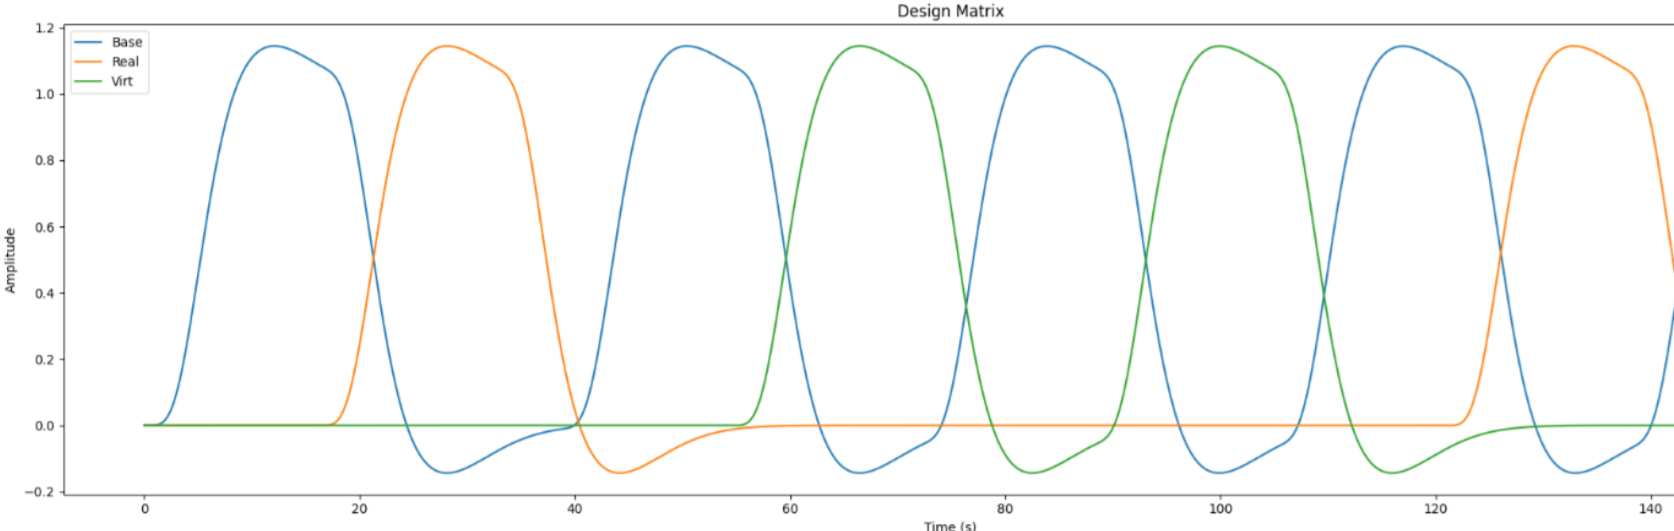
\includegraphics[width=1\textwidth]{C:/Users/super/OneDrive - Ontario Tech University/fNIRS_Emotions/plots/figures/Sample Design Matrix.png}
        \caption{Design matrix for a single participant (first 150s). Each condition is represented by a different color and represents the onset of a block.}
    \end{figure}
\end{frame}

% display C:\Users\super\OneDrive - Ontario Tech University\fNIRS_Emotions\plots\glm\group_results\results_face_type.png
\begin{frame}{GLM Analysis}
    \begin{itemize}
      \item \textbf{First-Level GLM:}
        \begin{itemize}
          \item Fit GLM per recording to estimate condition-specific responses.
          \item Extract both channel-level and ROI estimates.
        \end{itemize}
      \item \textbf{Group-Level Analysis:} $\theta \sim -1 + \text{ROI}:\text{Condition}:\text{Chroma}$
        \begin{itemize}
            \item This mixed effects model estimates separate coefficients ($\theta$'s) for each combination of ROI, condition, and channel type without a global intercept. 
            \item Group by participant for variability between subjects.
        \end{itemize}
    \end{itemize}
    \begin{figure}
        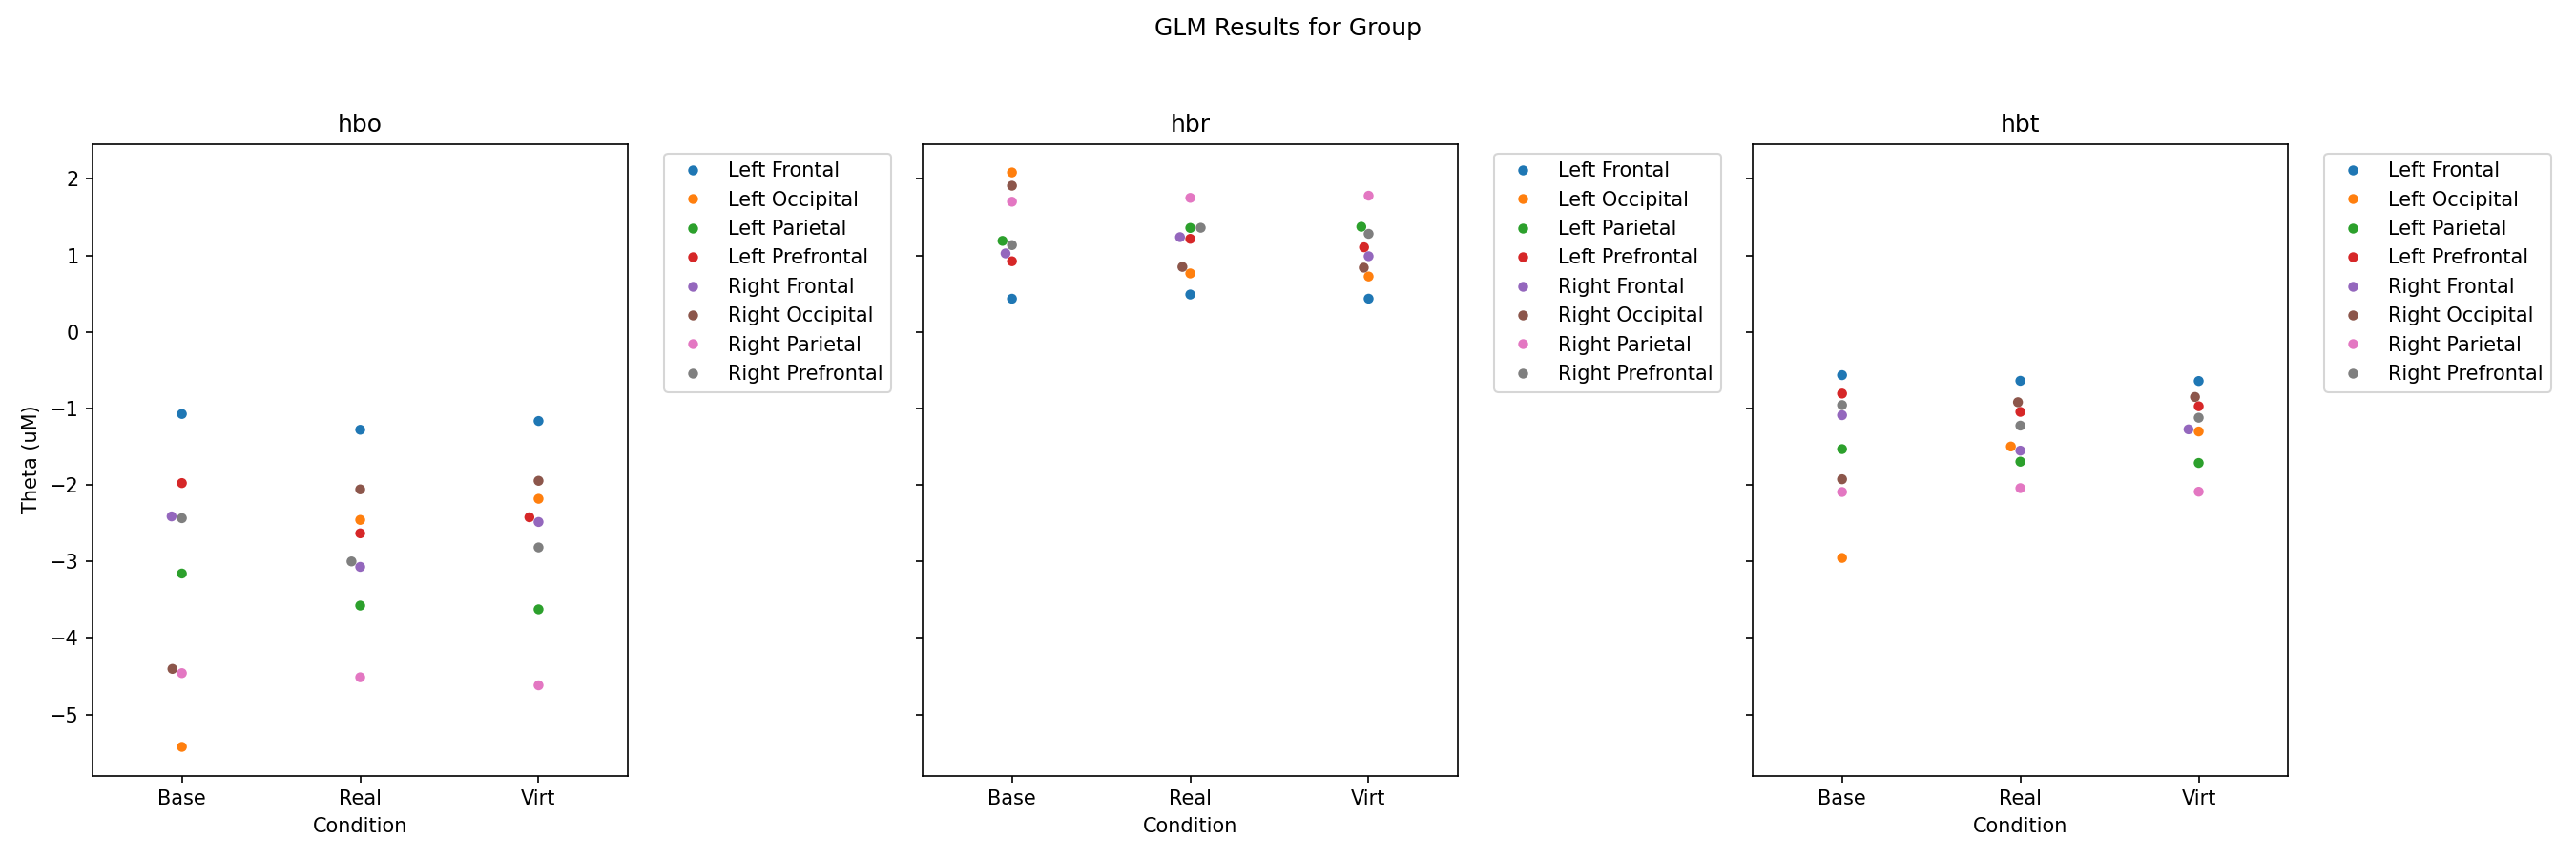
\includegraphics[width=0.9\textwidth]{C:/Users/super/OneDrive - Ontario Tech University/fNIRS_Emotions/plots/glm/group_results/results_face_type.png}
        \caption{Swarm plots display $\theta$'s across conditions/ROIs for each channel type. Higher $\theta$ values indicate stronger responses.}
    \end{figure}
\end{frame}

% display C:\Users\super\OneDrive - Ontario Tech University\fNIRS_Emotions\plots\glm\contrasts\differences\Contrast_Real-Virt.png
% display C:\Users\super\OneDrive - Ontario Tech University\fNIRS_Emotions\plots\glm\contrasts\differences\Contrast_Real-Base.png
% display C:\Users\super\OneDrive - Ontario Tech University\fNIRS_Emotions\plots\glm\contrasts\differences\Contrast_Anger-Surprise.png
% display these three side by side
\begin{frame}
    \frametitle{GLM Contrasts}
    \begin{itemize}
        \item \textbf{Contrasts:}
        \begin{itemize}
            \item Contrasts between pairs of conditions (i.e. \texttt{Joy - Fear}) are defined by subtracting corresponding regressors. 
            \item This highlights the differences in haemodynamic responses under the combinations of conditions.
        \end{itemize}
    \end{itemize}
    \begin{minipage}[t]{0.3\textwidth}
        \vspace{-\baselineskip}
        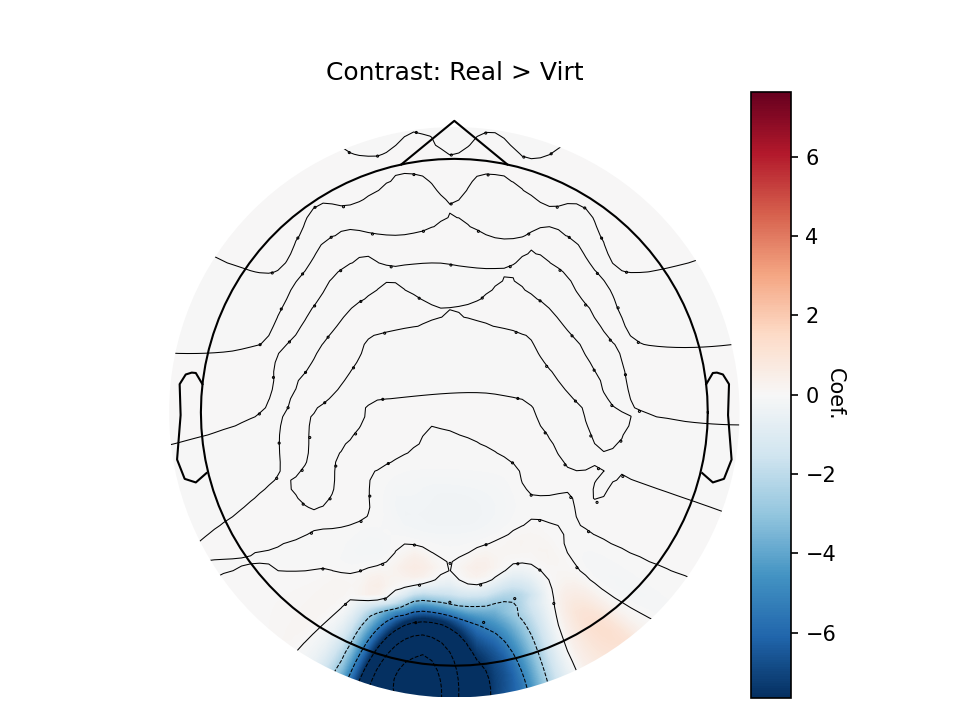
\includegraphics[width=\textwidth, trim=400 0 400 0, clip]{C:/Users/super/OneDrive - Ontario Tech University/fNIRS_Emotions/plots/glm/contrasts/differences/Contrast_Real-Virt.png}
    \end{minipage}
    \begin{minipage}[t]{0.3\textwidth}
        \vspace{-\baselineskip}
        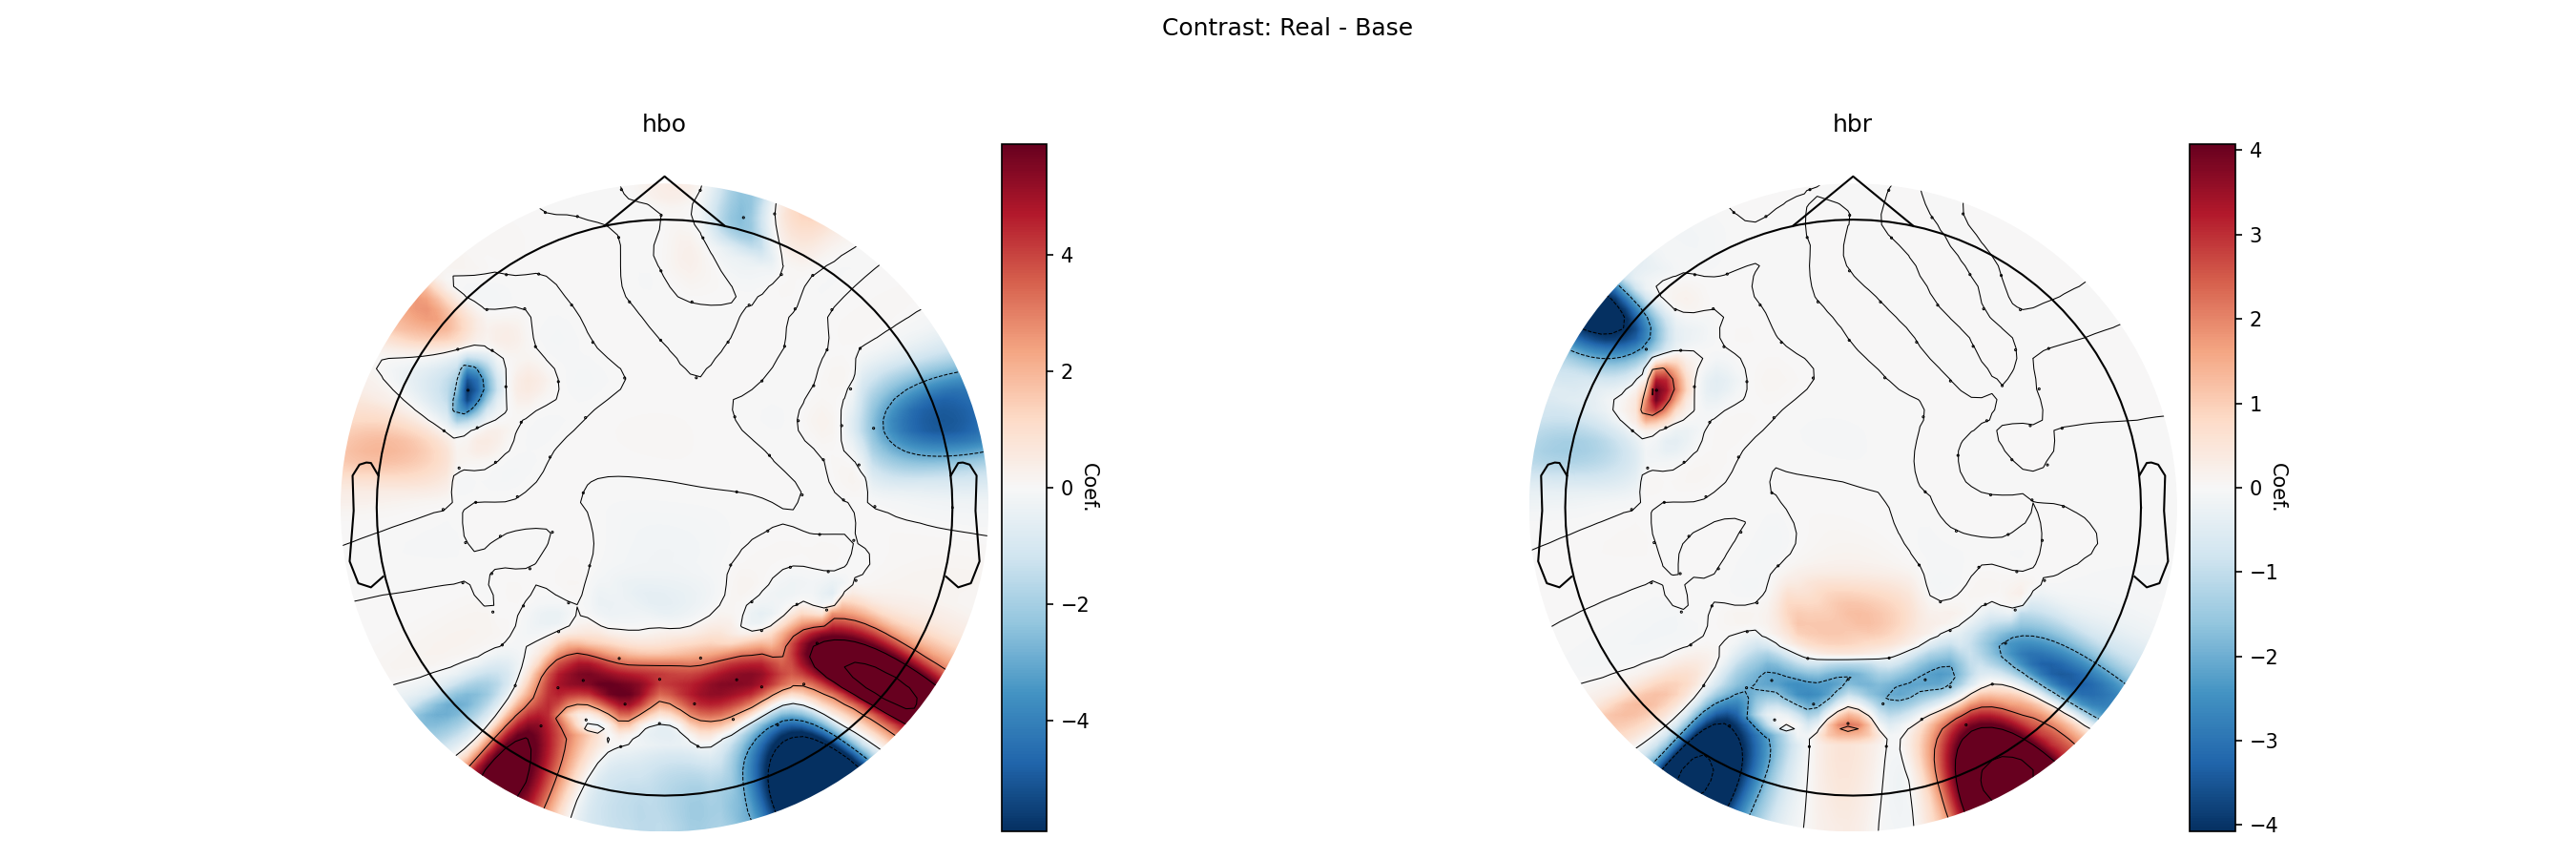
\includegraphics[width=\textwidth, trim=400 0 400 0, clip]{C:/Users/super/OneDrive - Ontario Tech University/fNIRS_Emotions/plots/glm/contrasts/differences/Contrast_Real-Base.png}
    \end{minipage}
    \begin{minipage}[t]{0.3\textwidth}
        \vspace{-\baselineskip}
        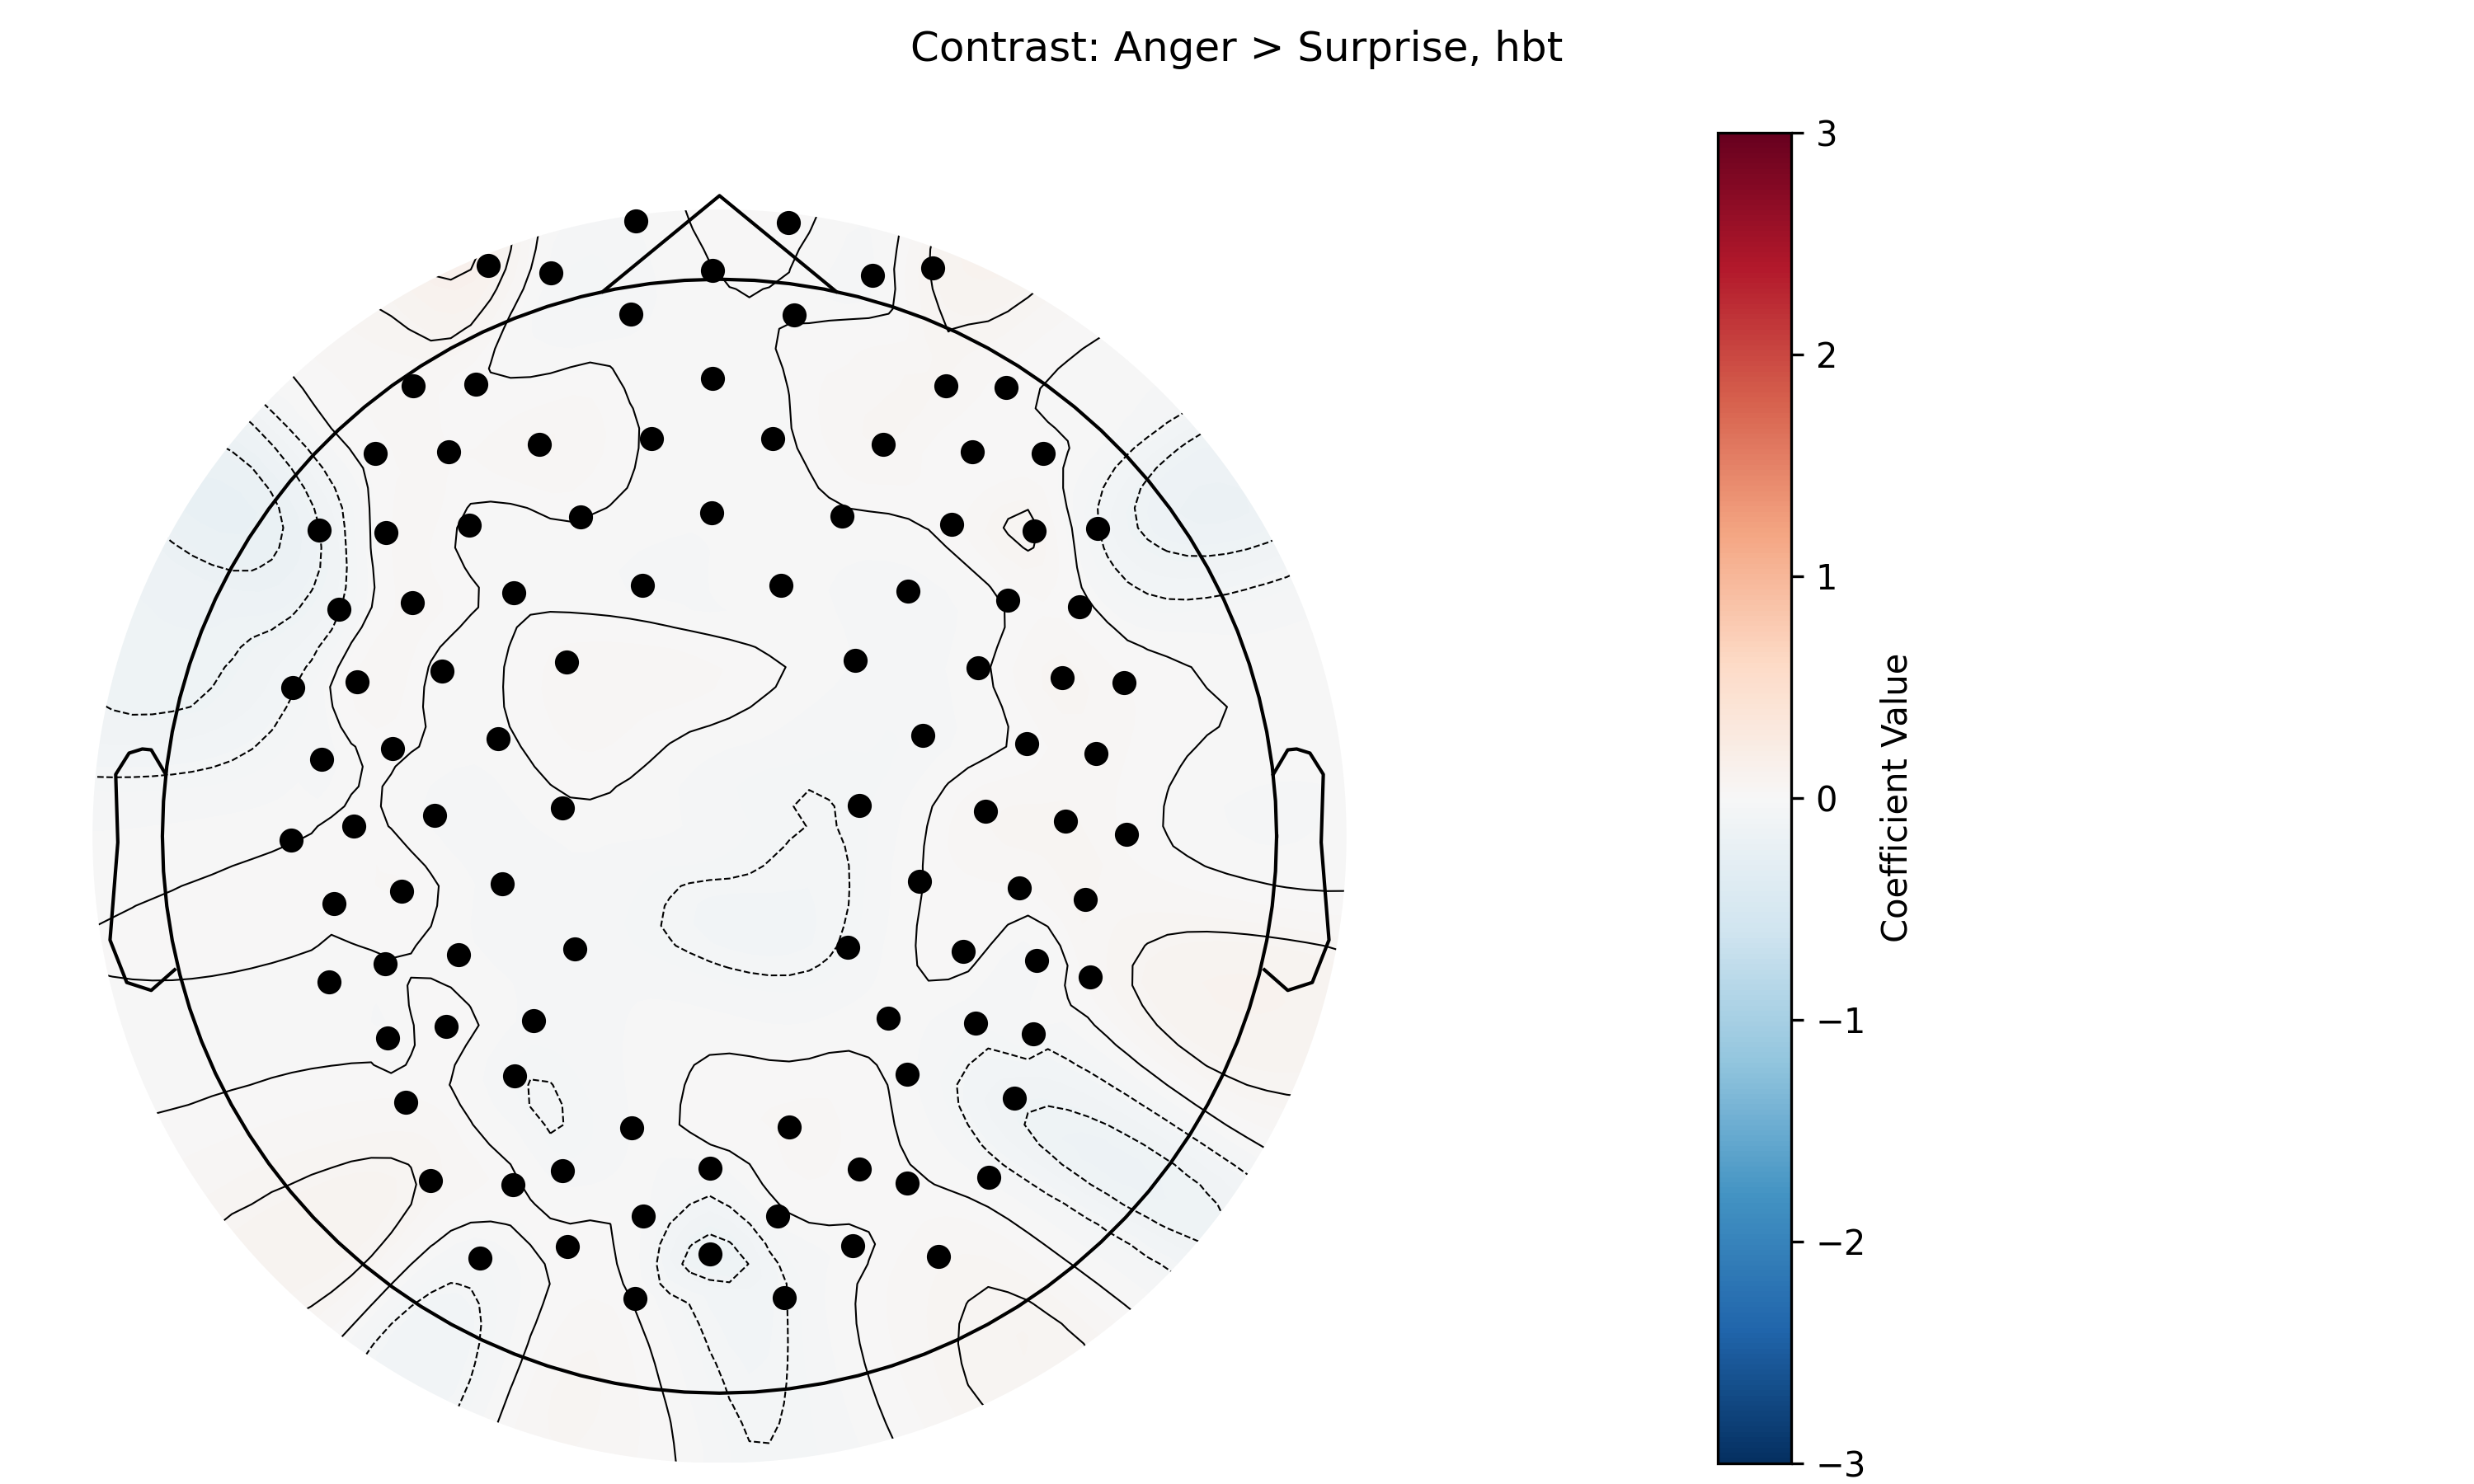
\includegraphics[width=\textwidth, trim=400 0 400 0, clip]{C:/Users/super/OneDrive - Ontario Tech University/fNIRS_Emotions/plots/glm/contrasts/differences/Contrast_Anger-Surprise.png}
    \end{minipage}
    \begin{figure}
        \caption{Contrast maps (Hbo) for Real vs. Virtual (left), Real vs. Baseline (middle), and Anger vs. Surprise (right).}
        \begin{itemize}
            \item Only channels with \(P < |z|\) greater than 0.05 are displayed, indicating a significant difference in Hbo.
        \end{itemize}
    \end{figure}
\end{frame}

% display C:\Users\super\OneDrive - Ontario Tech University\fNIRS_Emotions\plots\erp\erp_conditions\Real.png
\begin{frame}
    \frametitle{Event Related Potentials (ERPs)}
    \begin{figure}
        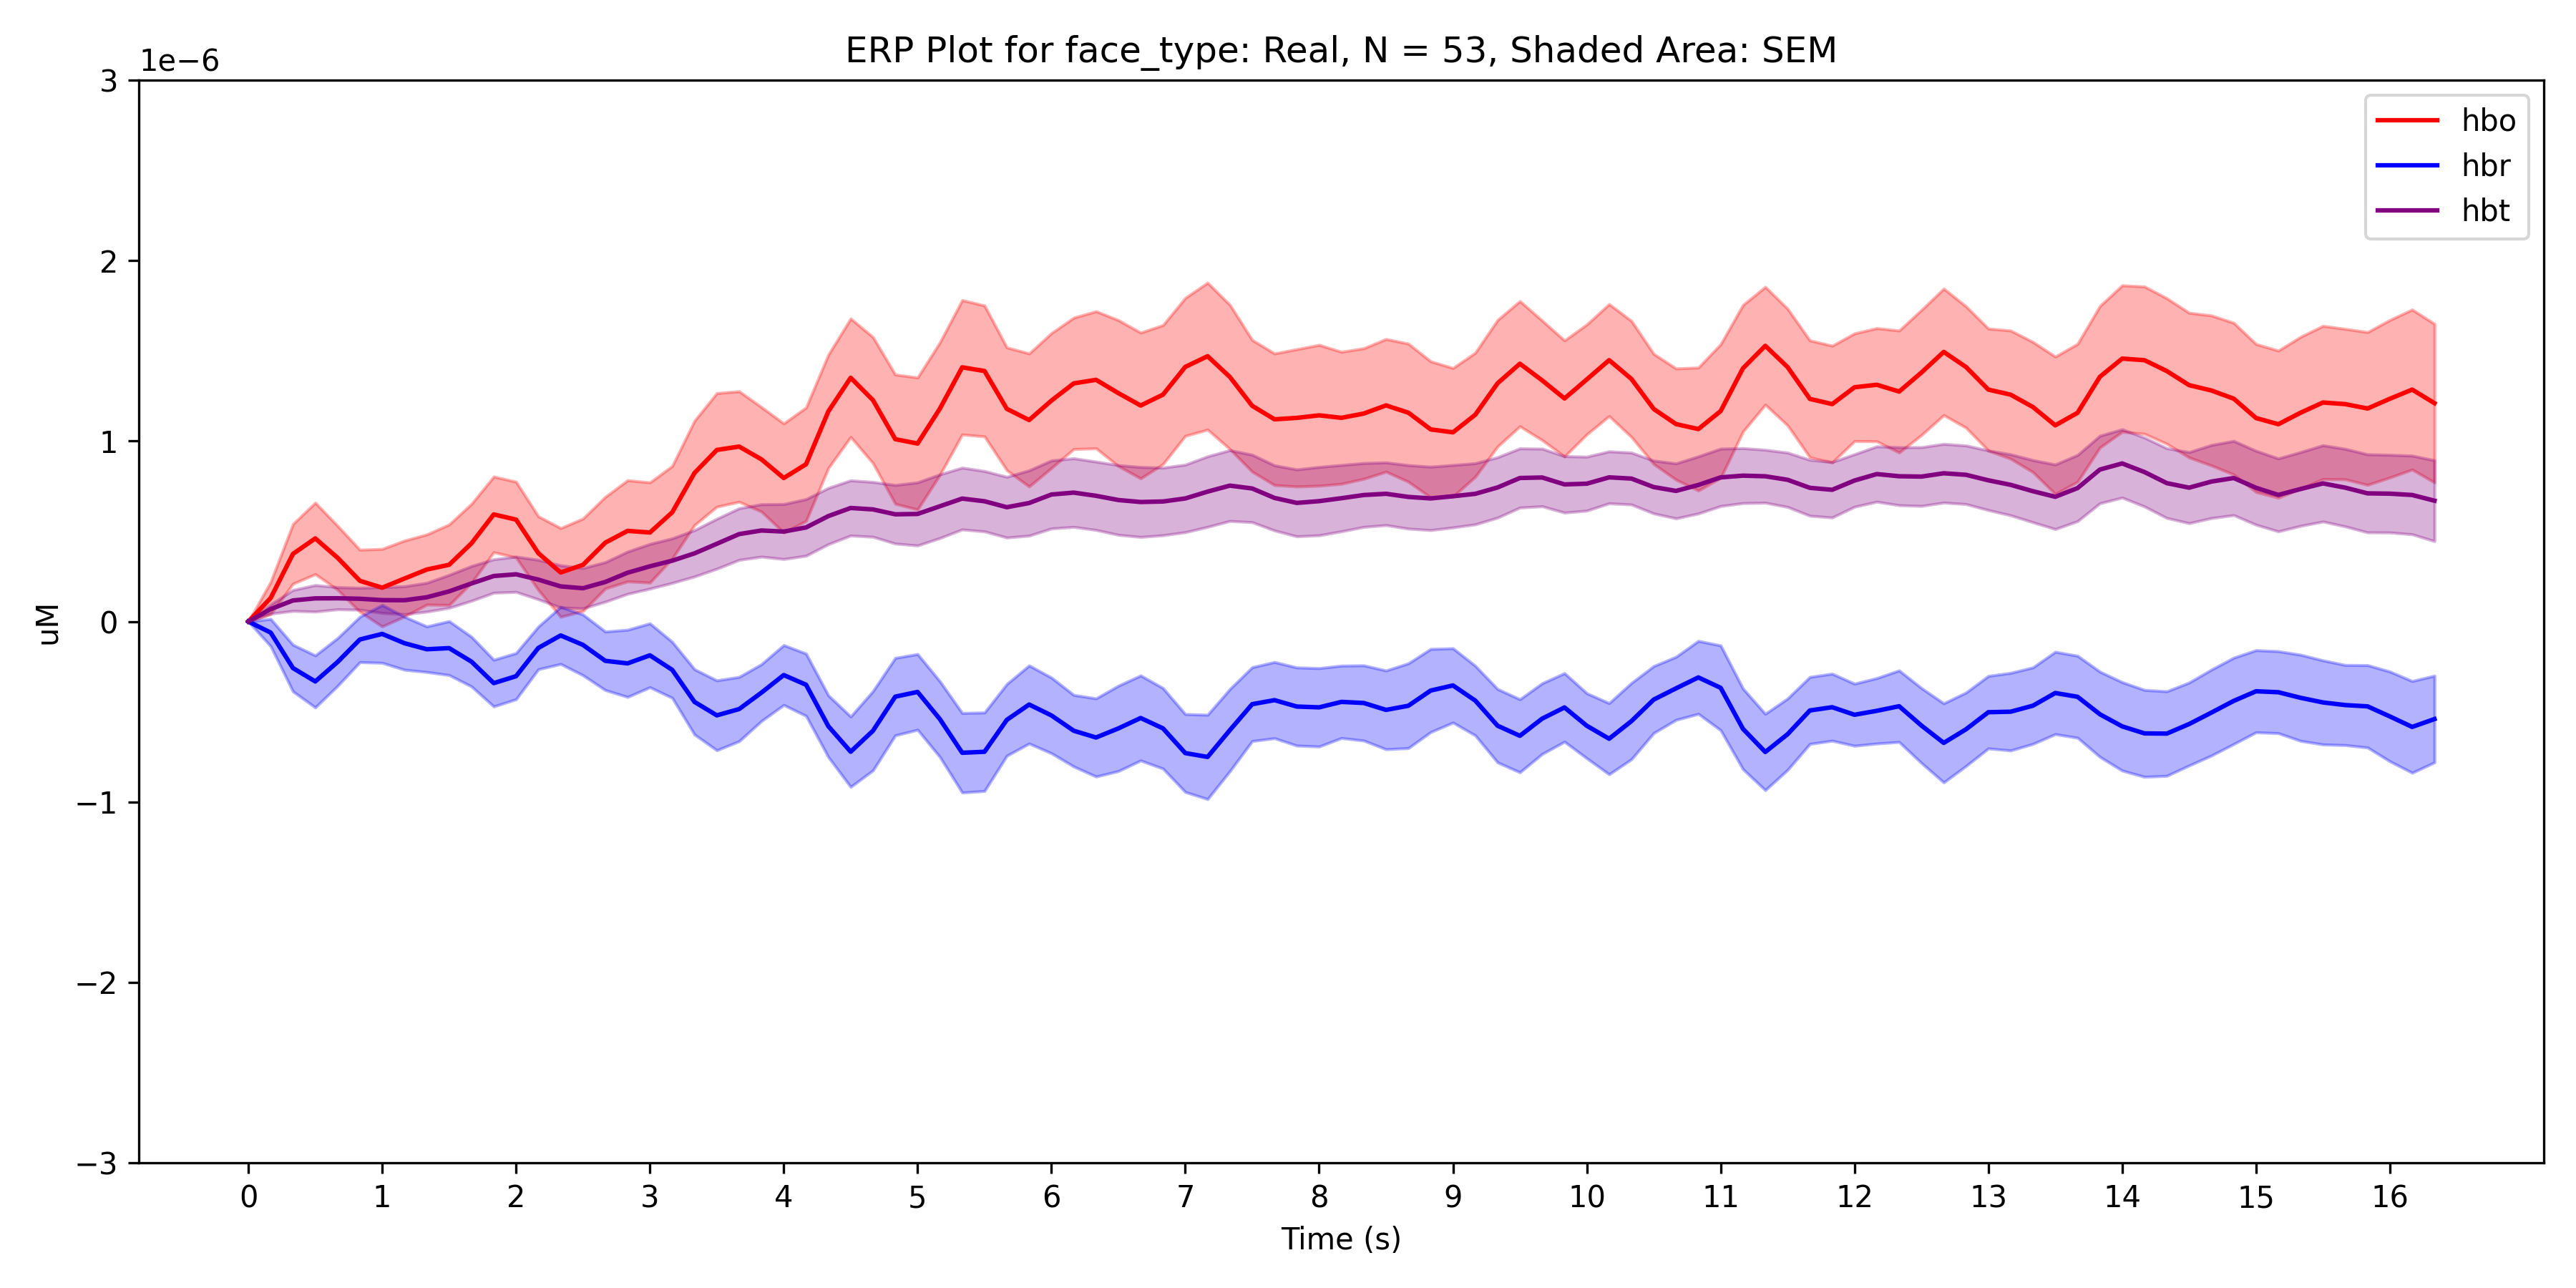
\includegraphics[width=0.9\textwidth]{C:/Users/super/OneDrive - Ontario Tech University/fNIRS_Emotions/plots/erp/erp_conditions/Real.png}
        \caption{ERP for real face epochs across all channels. The x-axis represents time in seconds ($s$) and the y-axis represents the $\Delta$Hbo/Hbr/Hbt in micromolars ($\mu M$).}
        \begin{itemize}
            \item The shaded region is the standard error of the mean (SEM): $\frac{\sigma}{\sqrt{n}}$. 
        \end{itemize}
    \end{figure}
\end{frame}

% display C:\Users\super\OneDrive - Ontario Tech University\fNIRS_Emotions\plots\erp\erp_differences\Fear_Sadness.png
\begin{frame}
    \frametitle{ERP Differences}
    \begin{figure}
        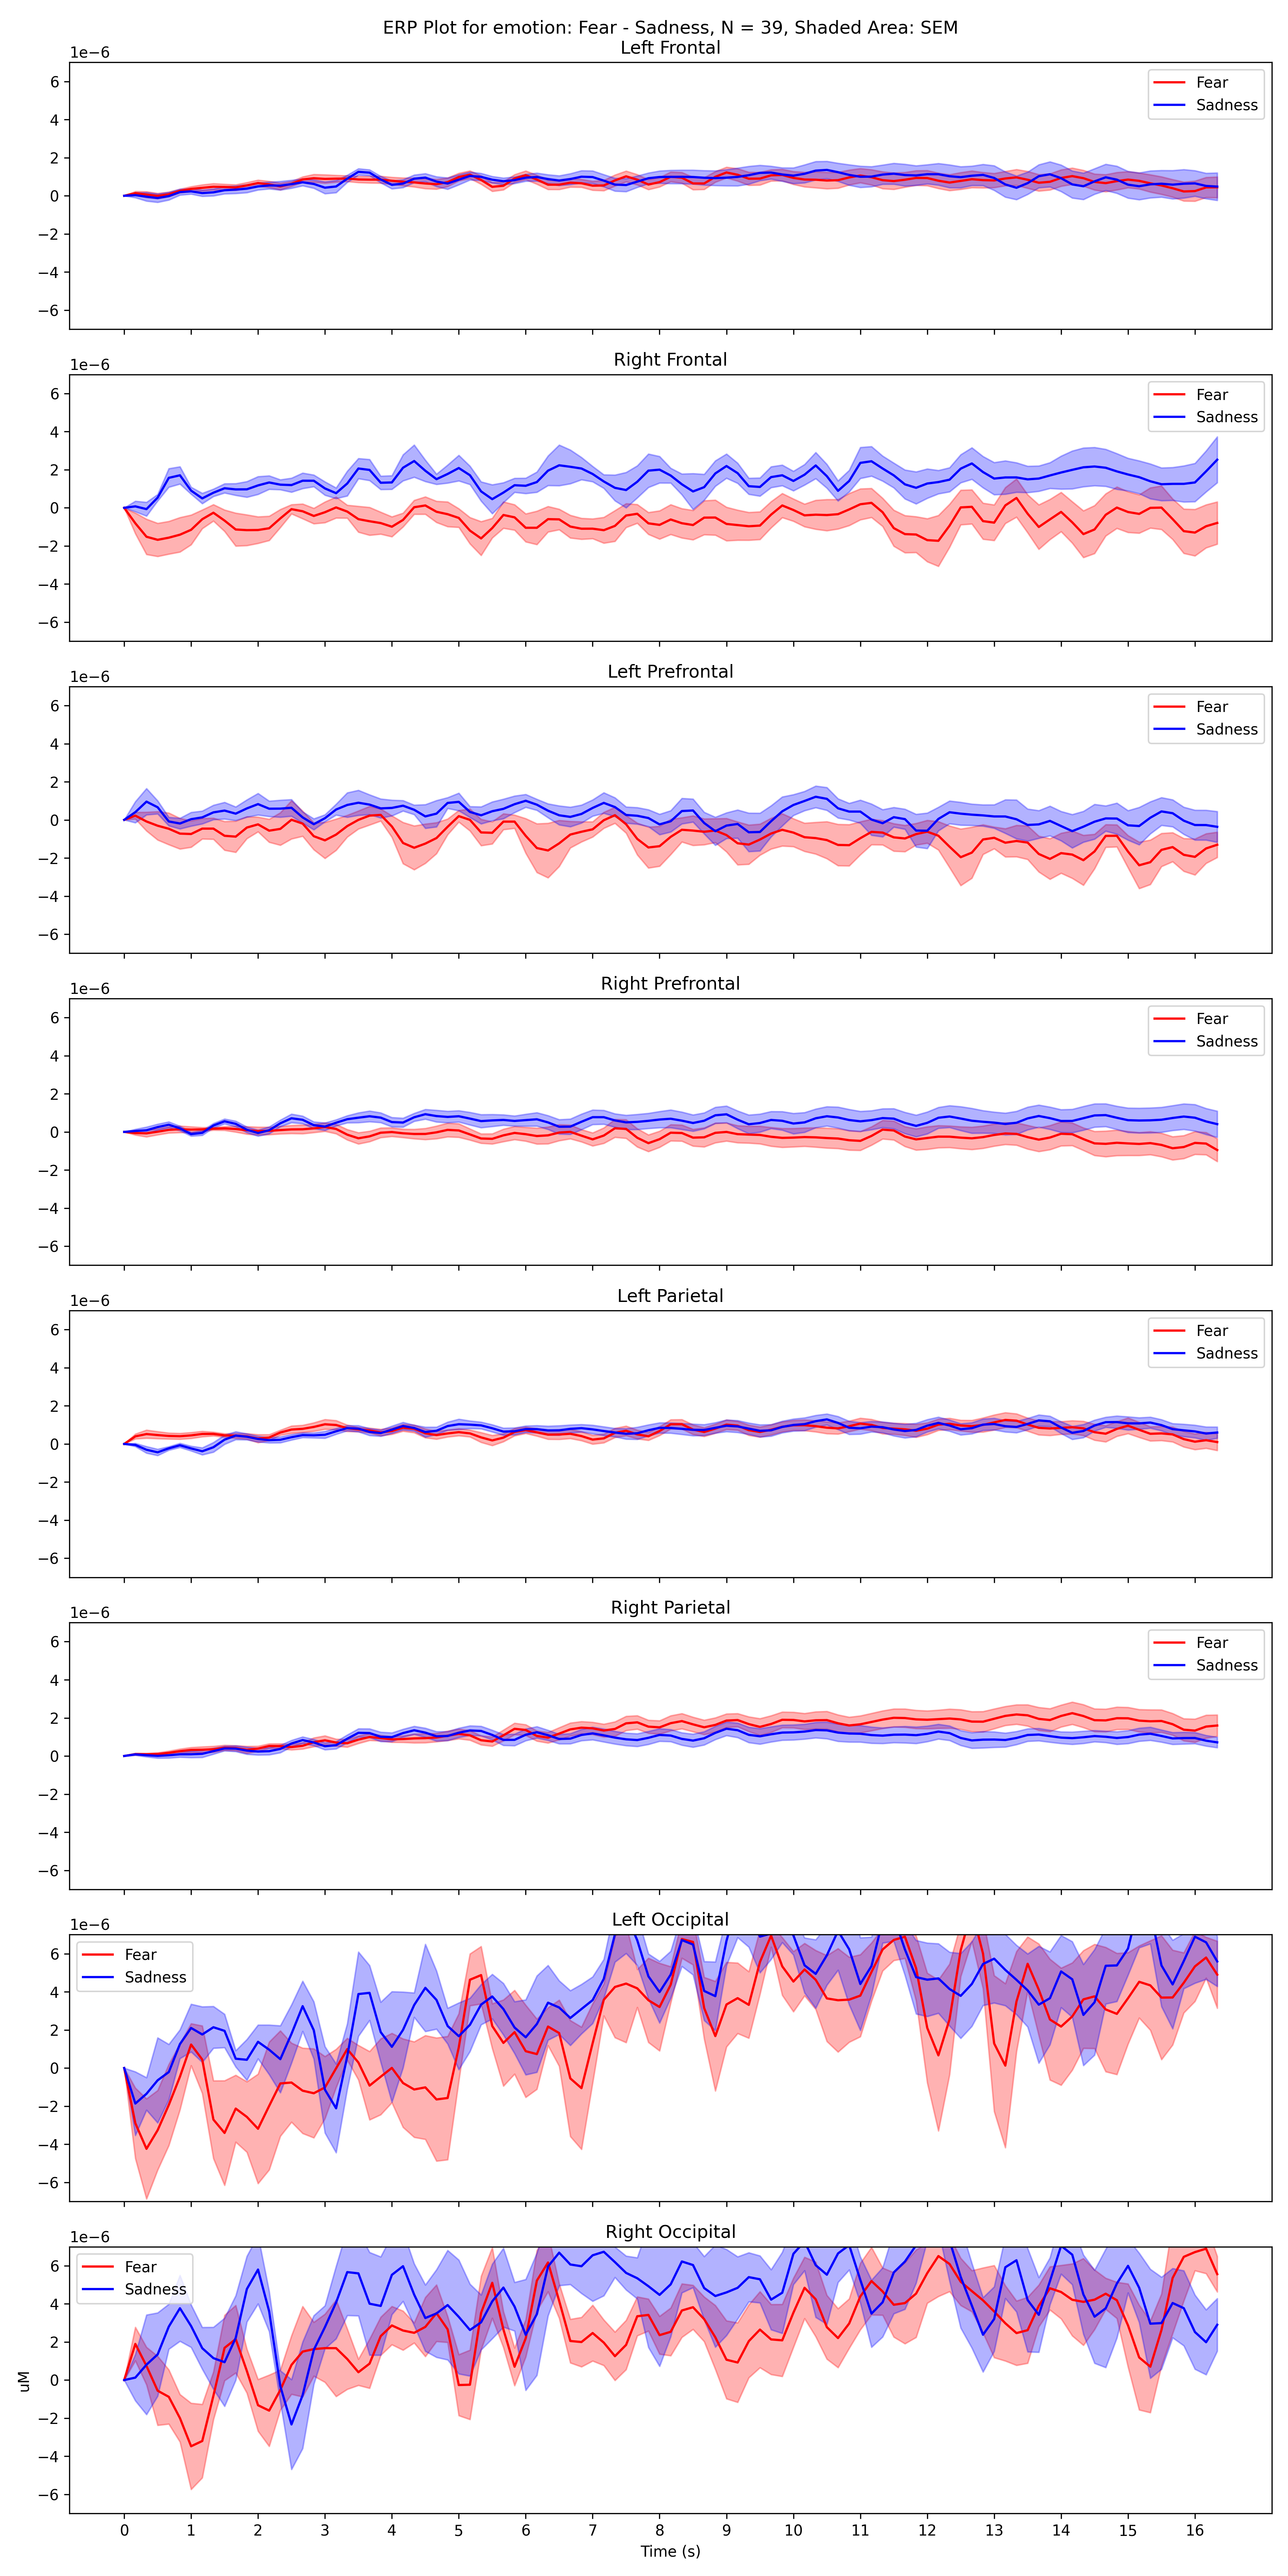
\includegraphics[width=1\textwidth, trim=0 1290 0 0, clip]{C:/Users/super/OneDrive - Ontario Tech University/fNIRS_Emotions/plots/erp/erp_differences/Fear_Sadness.png}
        \caption{ERP difference in Hbo between fear and sadness for Left/Right frontal regions. }
    \end{figure}
\end{frame}

% display C:\Users\super\OneDrive - Ontario Tech University\fNIRS_Emotions\plots\erp\erp_differences\Fear_Sadness.png
\begin{frame}
    \frametitle{ERP Differences}
    \begin{figure}
        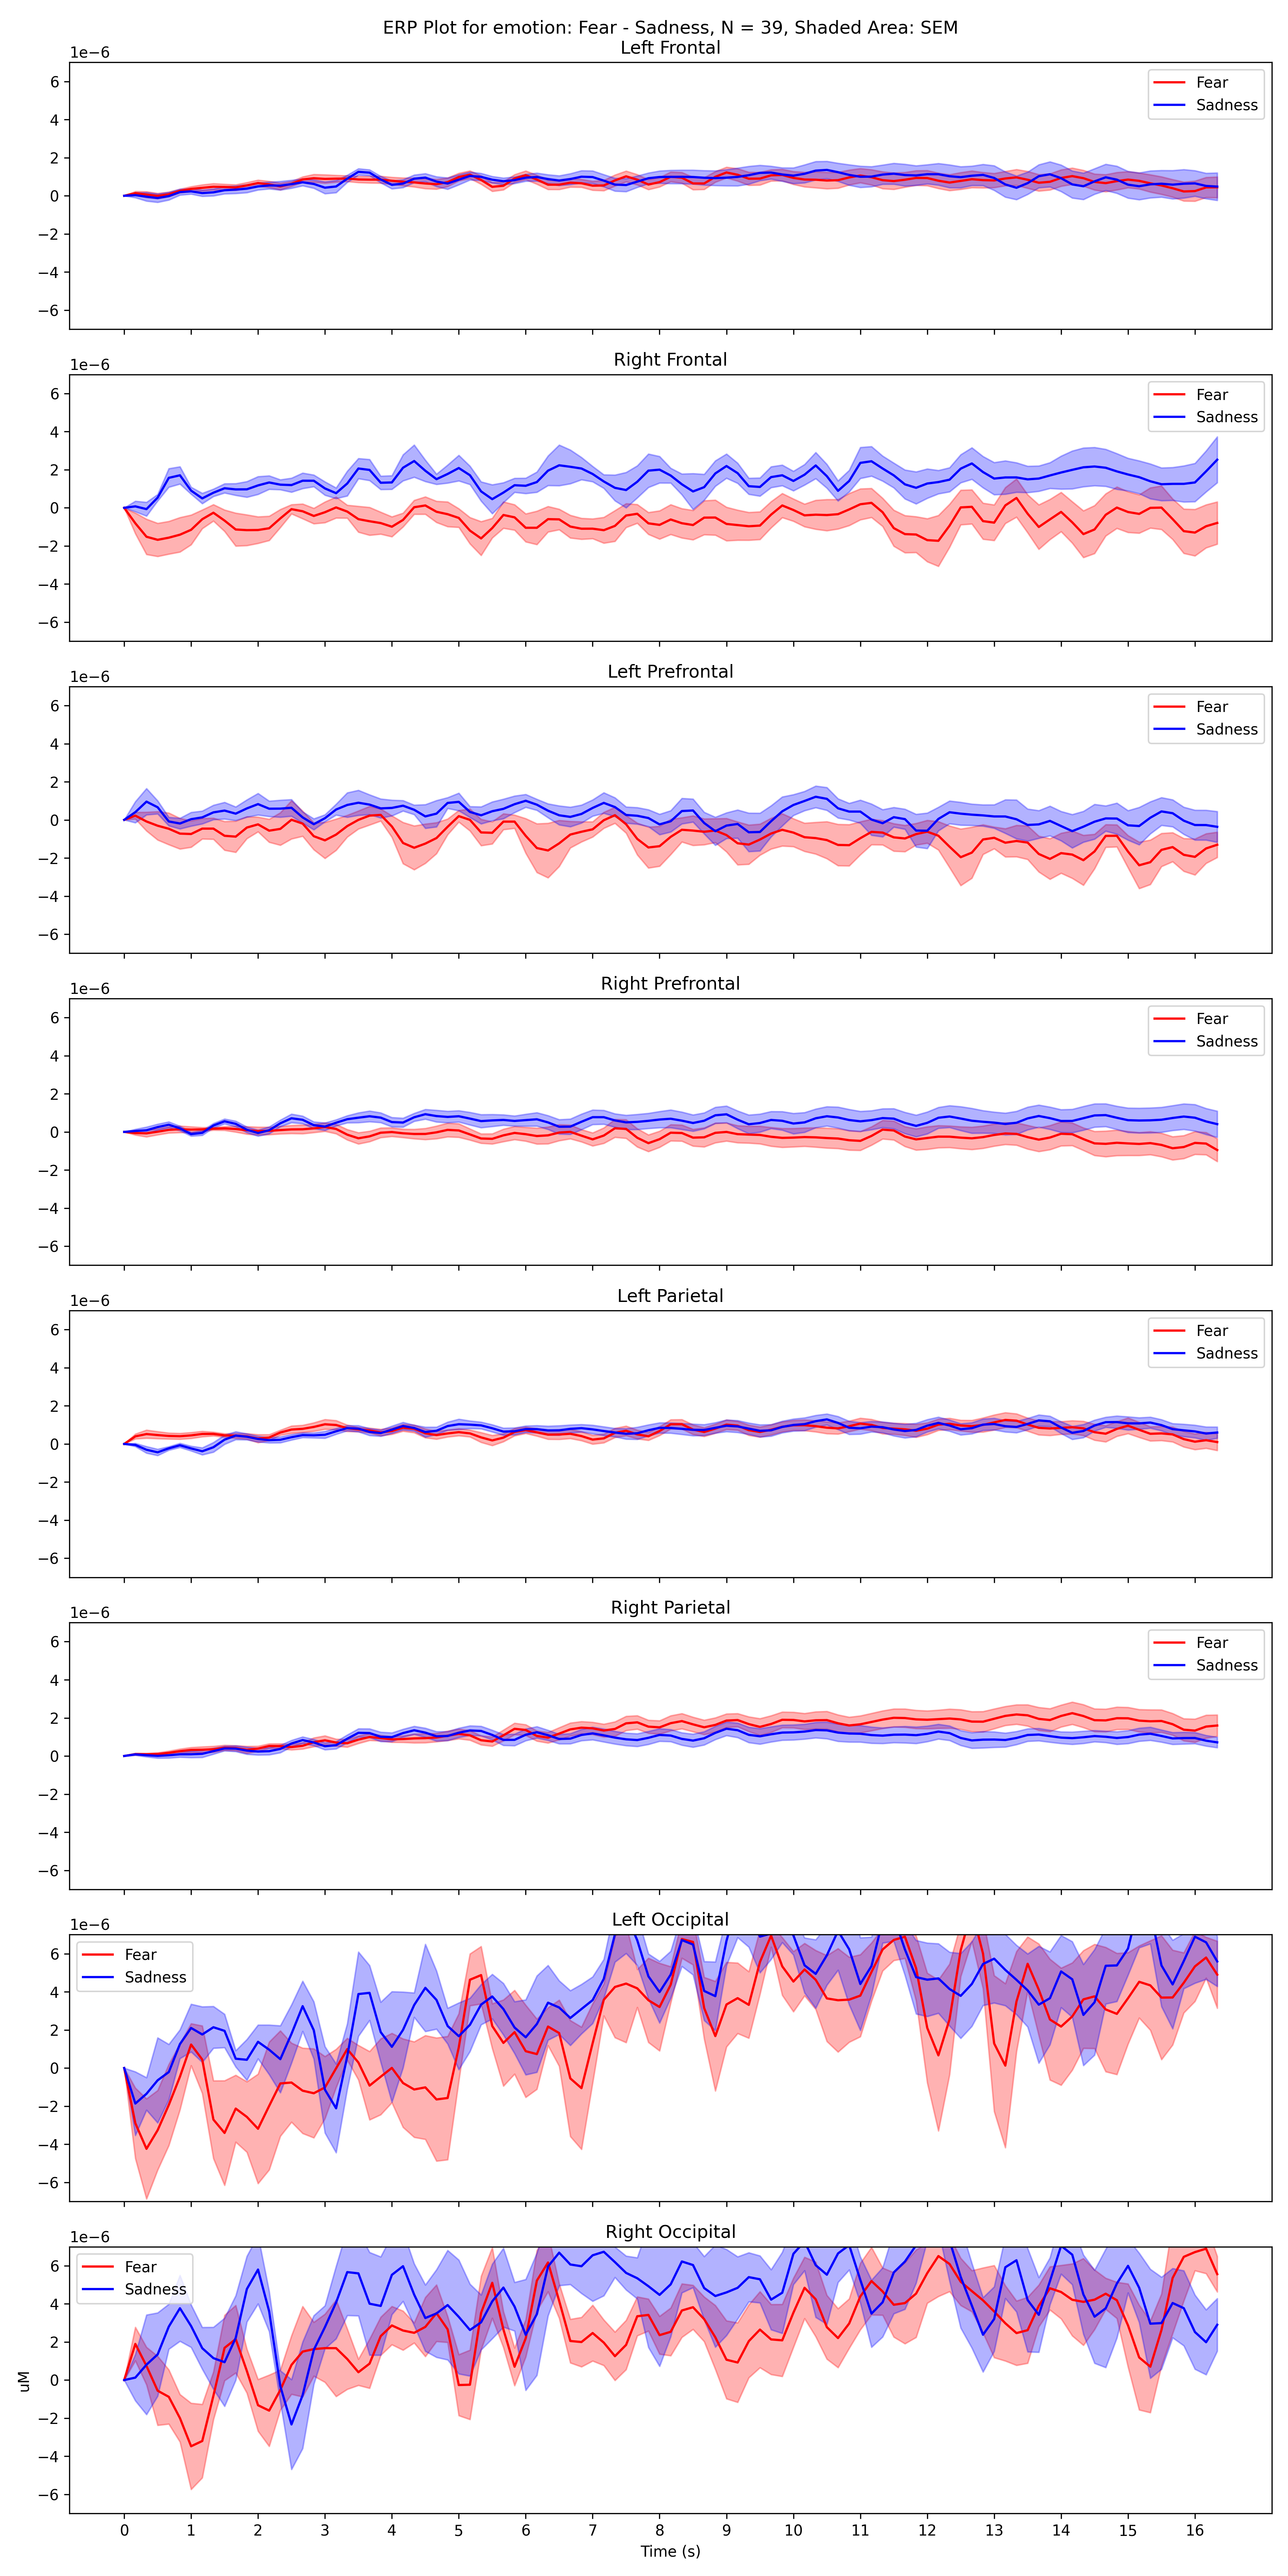
\includegraphics[width=1\textwidth, trim=0 0 0 1275, clip]{C:/Users/super/OneDrive - Ontario Tech University/fNIRS_Emotions/plots/erp/erp_differences/Fear_Sadness.png}
        \caption{ERP difference in Hbo between fear and sadness for Left/Right occipital regions. }
    \end{figure}
\end{frame}

\begin{frame}
    \frametitle{Connectivity Analysis}
    \begin{itemize}
        \item \textbf{Connectivity Analysis:}
        \begin{itemize}
            \item Continuous Wavelet Transform with a Morlet wavelet to analyze the frequency-domain characteristics of the data.
            \item Connectivity matrices were computed resulting in a 5D \texttt{(num\_participants, num\_channel\_types, num\_channel\_connections, num\_frequencies, num\_times)} array for each condition. 
        \end{itemize}
        \item \textbf{Connectivity Parameters:}
             \begin{itemize}
                    \item \texttt{\textcolor{blue}{channel\_types} = ['hbo', 'hbr', 'hbt'] \textcolor[rgb]{0.0, 0.5, 0.0}{\# channel types to analyze}}
                    \item \texttt{\textcolor{blue}{method} = "coh" \textcolor[rgb]{0.0, 0.5, 0.0}{\# coherence is used as the connectivity metric}}
                    \item \texttt{\textcolor{blue}{con\_mode} = "cwt\_morlet" \textcolor[rgb]{0.0, 0.5, 0.0}{\# the morlet wavelet is used for the CWT}}
                    \item \texttt{\textcolor{blue}{cwt\_freqs} = np.linspace(0.01, 0.5, 10) \textcolor[rgb]{0.0, 0.5, 0.0}{\# Pick 10 evenly spaced frequencies between 0.01 and 0.5 Hz}}
                    \item \texttt{\textcolor{blue}{cwt\_n\_cycles} = 10 \textcolor[rgb]{0.0, 0.5, 0.0}{\# Number of cycles for the Morlet wavelet}}
                    \item \texttt{\textcolor{blue}{faverage} = True \textcolor[rgb]{0.0, 0.5, 0.0}{\# Average the connectivity matrices across frequencies}}
                \end{itemize}
    \end{itemize}
\end{frame}

% display C:\Users\super\OneDrive - Ontario Tech University\fNIRS_Emotions\plots\connectivity\heatmaps\individual\face_type_Virt_cons\con_31.png
% display C:\Users\super\OneDrive - Ontario Tech University\fNIRS_Emotions\plots\connectivity\heatmaps\conditions\face_type_Virt_con.png
% display these two side by side
\begin{frame}
    \frametitle{Connectivity Heatmaps}
    \begin{minipage}[t]{0.45\textwidth}
        \vspace{-\baselineskip}
        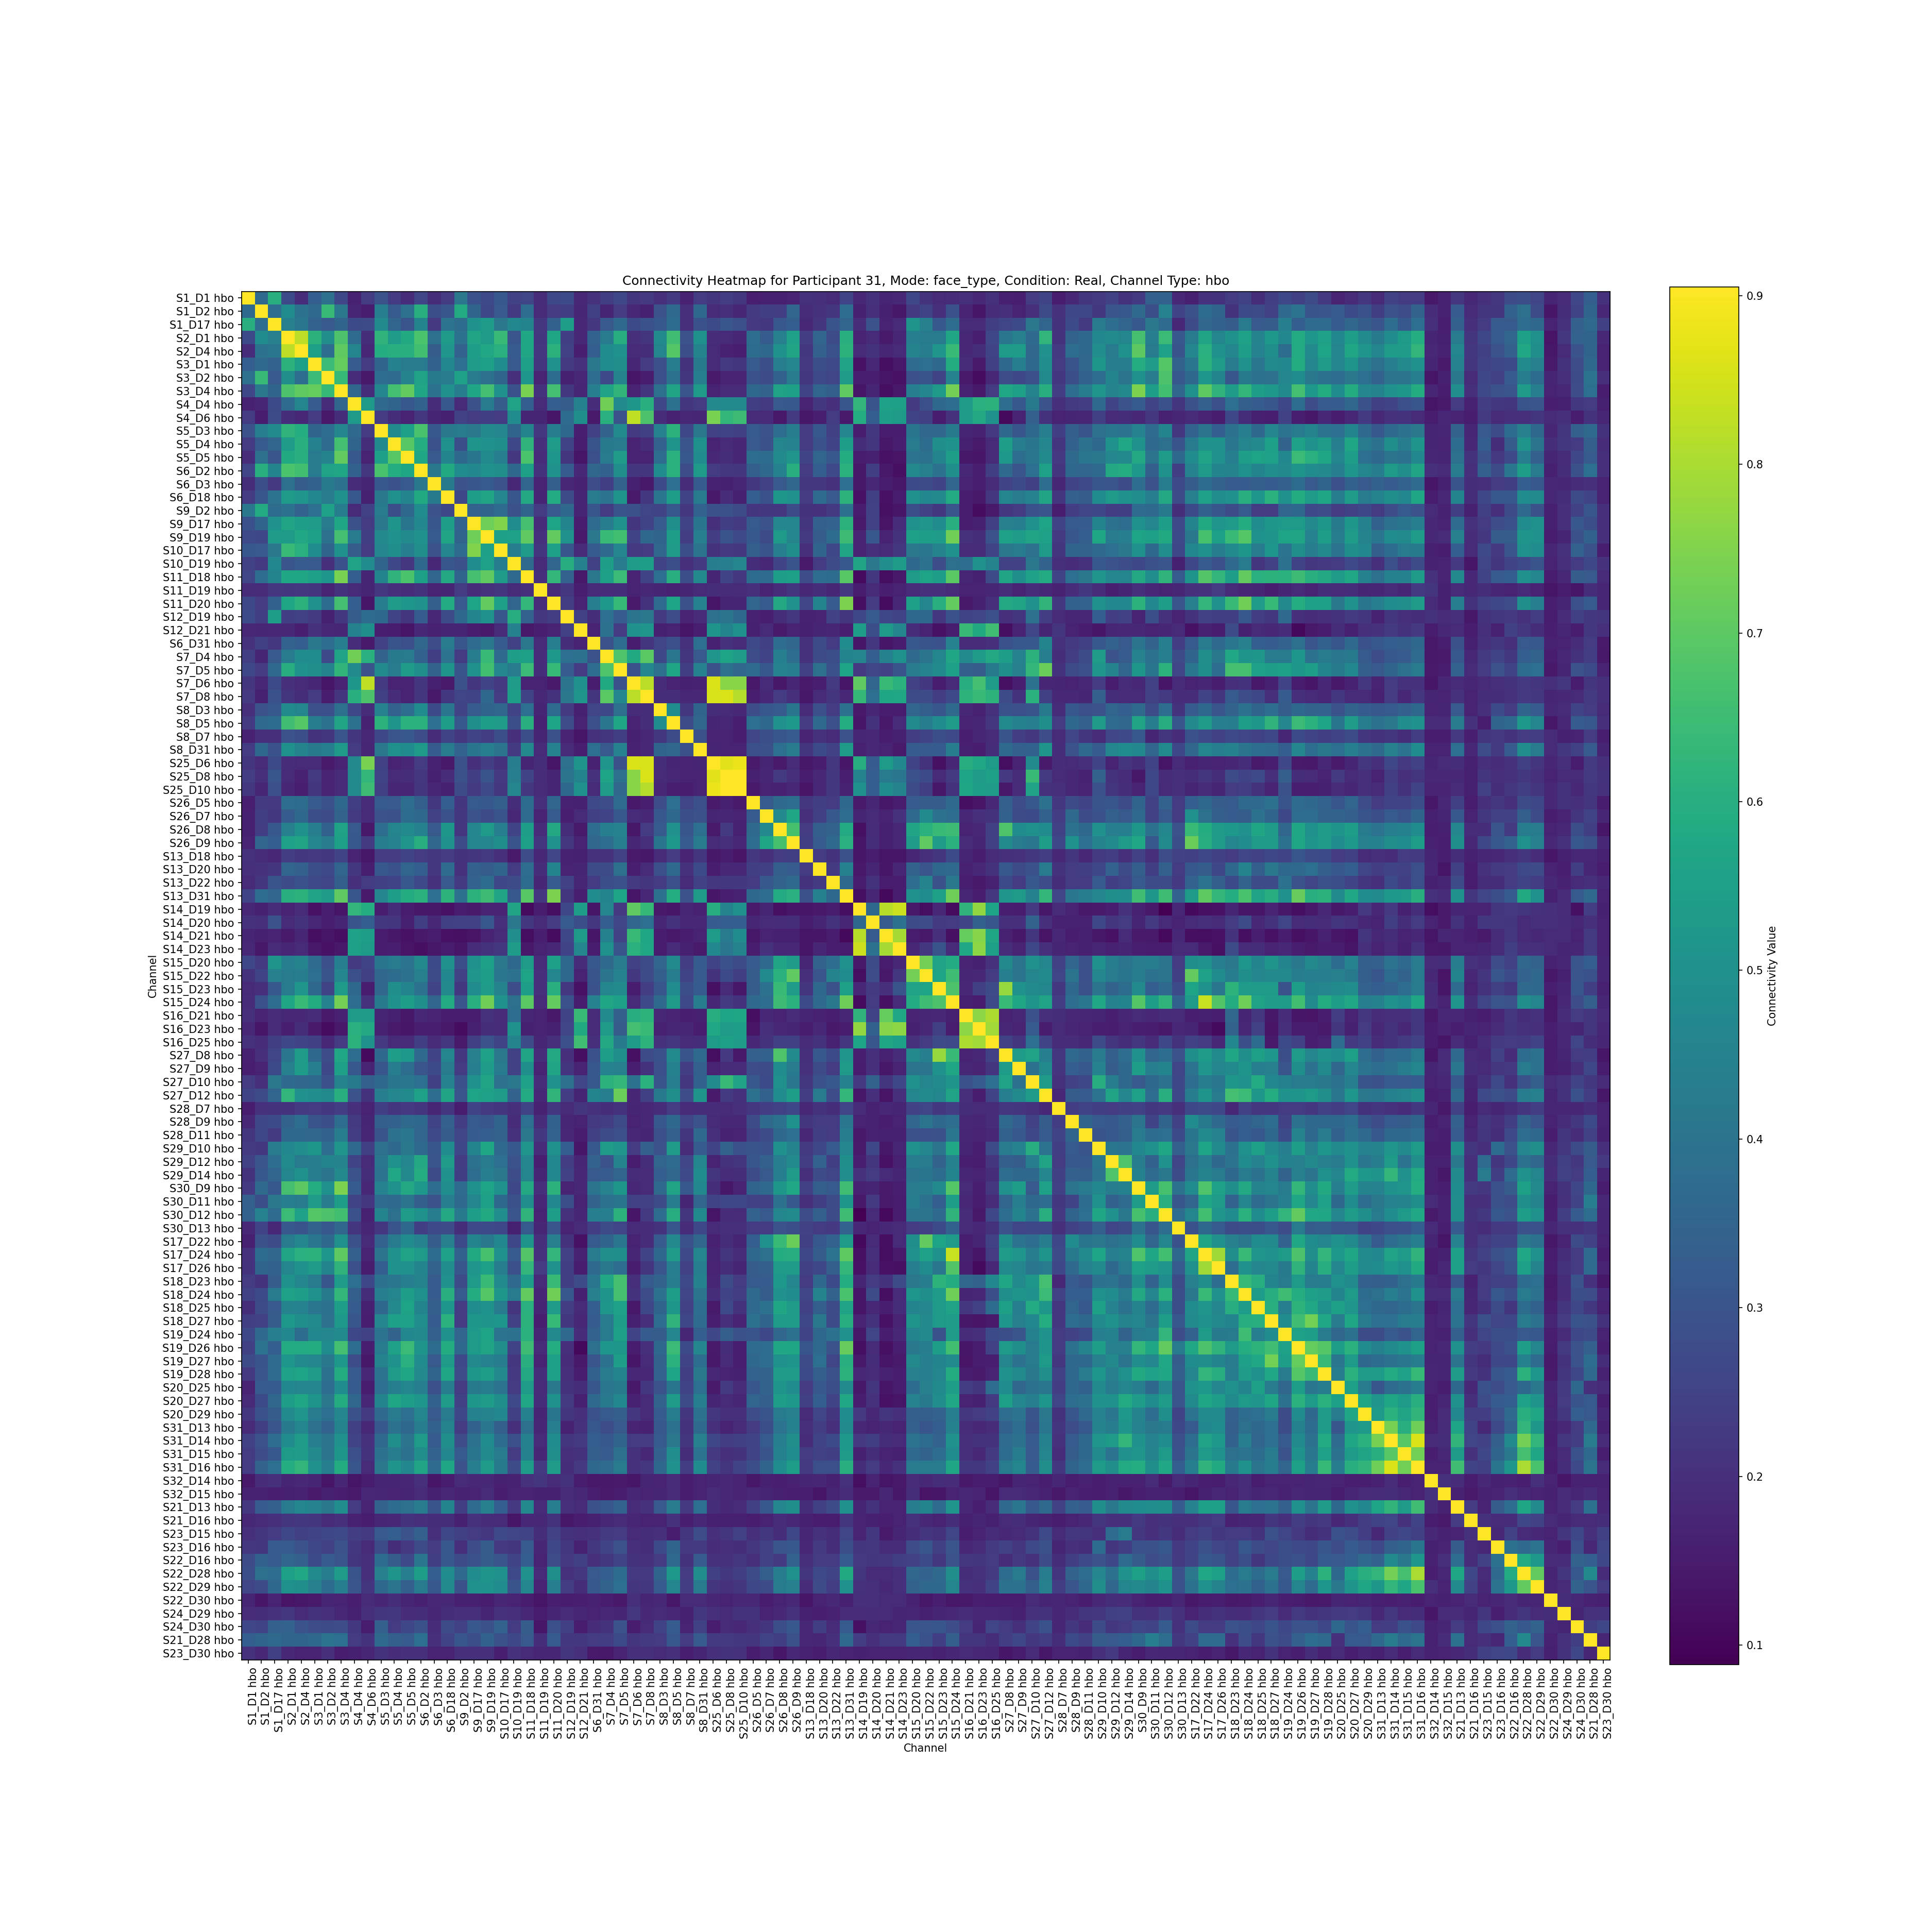
\includegraphics[width=\textwidth]{C:/Users/super/OneDrive - Ontario Tech University/fNIRS_Emotions/plots/connectivity/heatmaps/individual/face_type_Virt_cons/con_31.png}
    \end{minipage}
    \begin{minipage}[t]{0.45\textwidth}
        \vspace{-\baselineskip}
        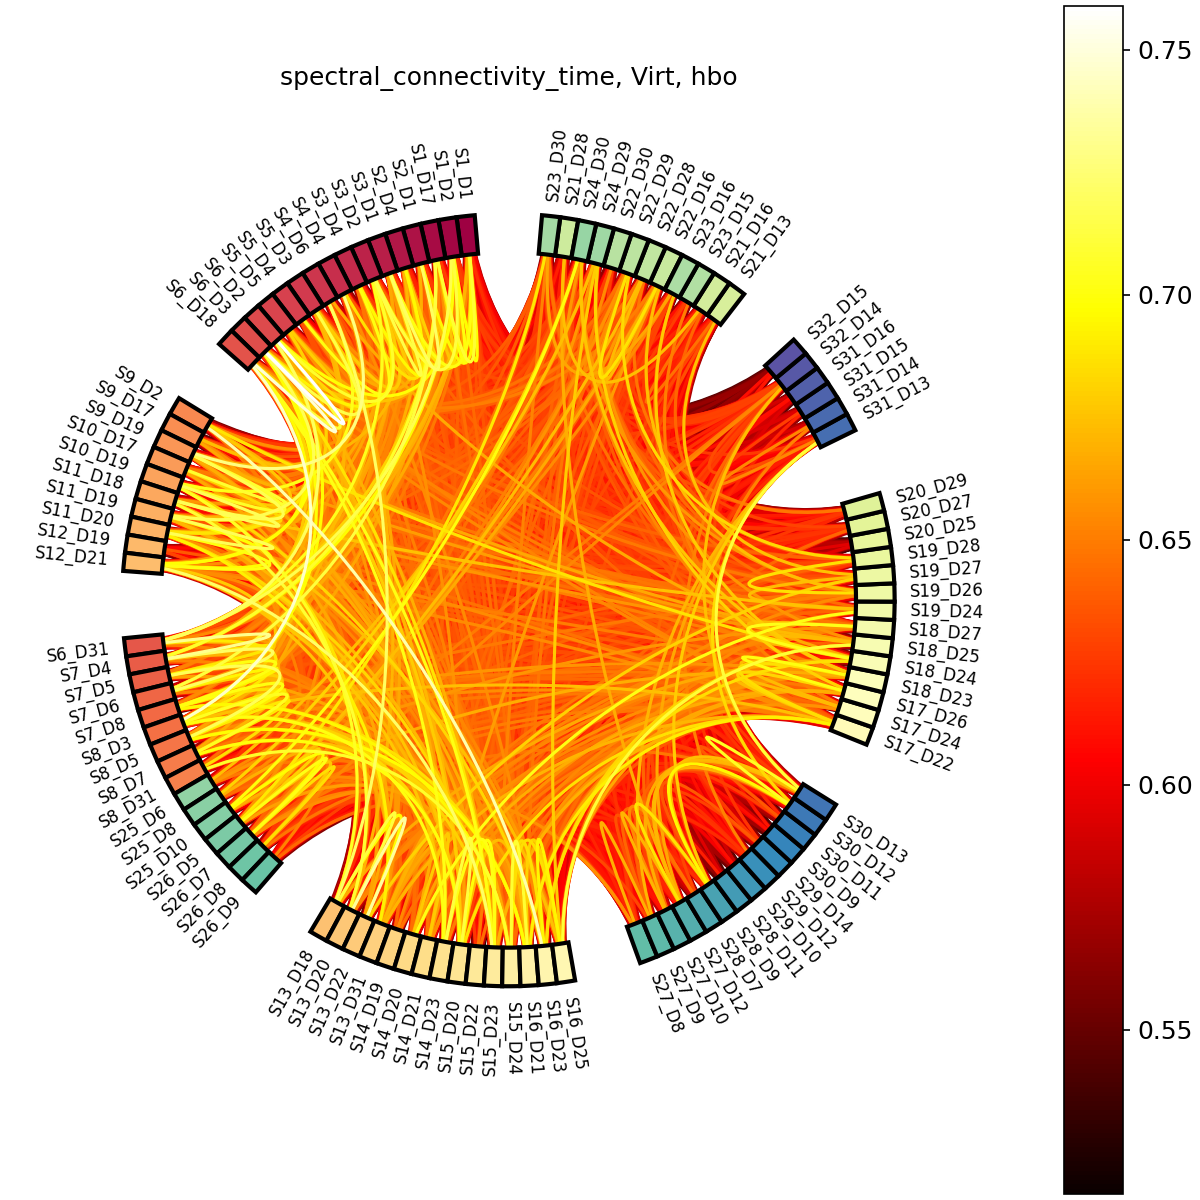
\includegraphics[width=\textwidth]{C:/Users/super/OneDrive - Ontario Tech University/fNIRS_Emotions/plots/connectivity/heatmaps/conditions/face_type_Virt_con.png}
    \end{minipage}
    \begin{figure}
        \caption{Virtual face connectivity heatmaps for a single participant (left) and the average across all participants (right).
        The x-axis and y-axis represent the channel number. A brighter color represents higher connectivity strength.}
        \begin{itemize}
            \item We can see that the average connectivity heatmap has a more washed out distribution of connectivity strength.
        \end{itemize}
    \end{figure}
\end{frame}

% display C:\Users\super\OneDrive - Ontario Tech University\fNIRS_Emotions\plots\connectivity\chord_plots\conditions\emotion_Sadness_con.png
% display C:\Users\super\OneDrive - Ontario Tech University\fNIRS_Emotions\plots\connectivity\chord_plots\conditions\face_type_Base_con.png
% display these two side by side
\begin{frame}
    \frametitle{Connectivity Chord Plots}
    \begin{minipage}[t]{0.45\textwidth}
        \vspace{-\baselineskip}
        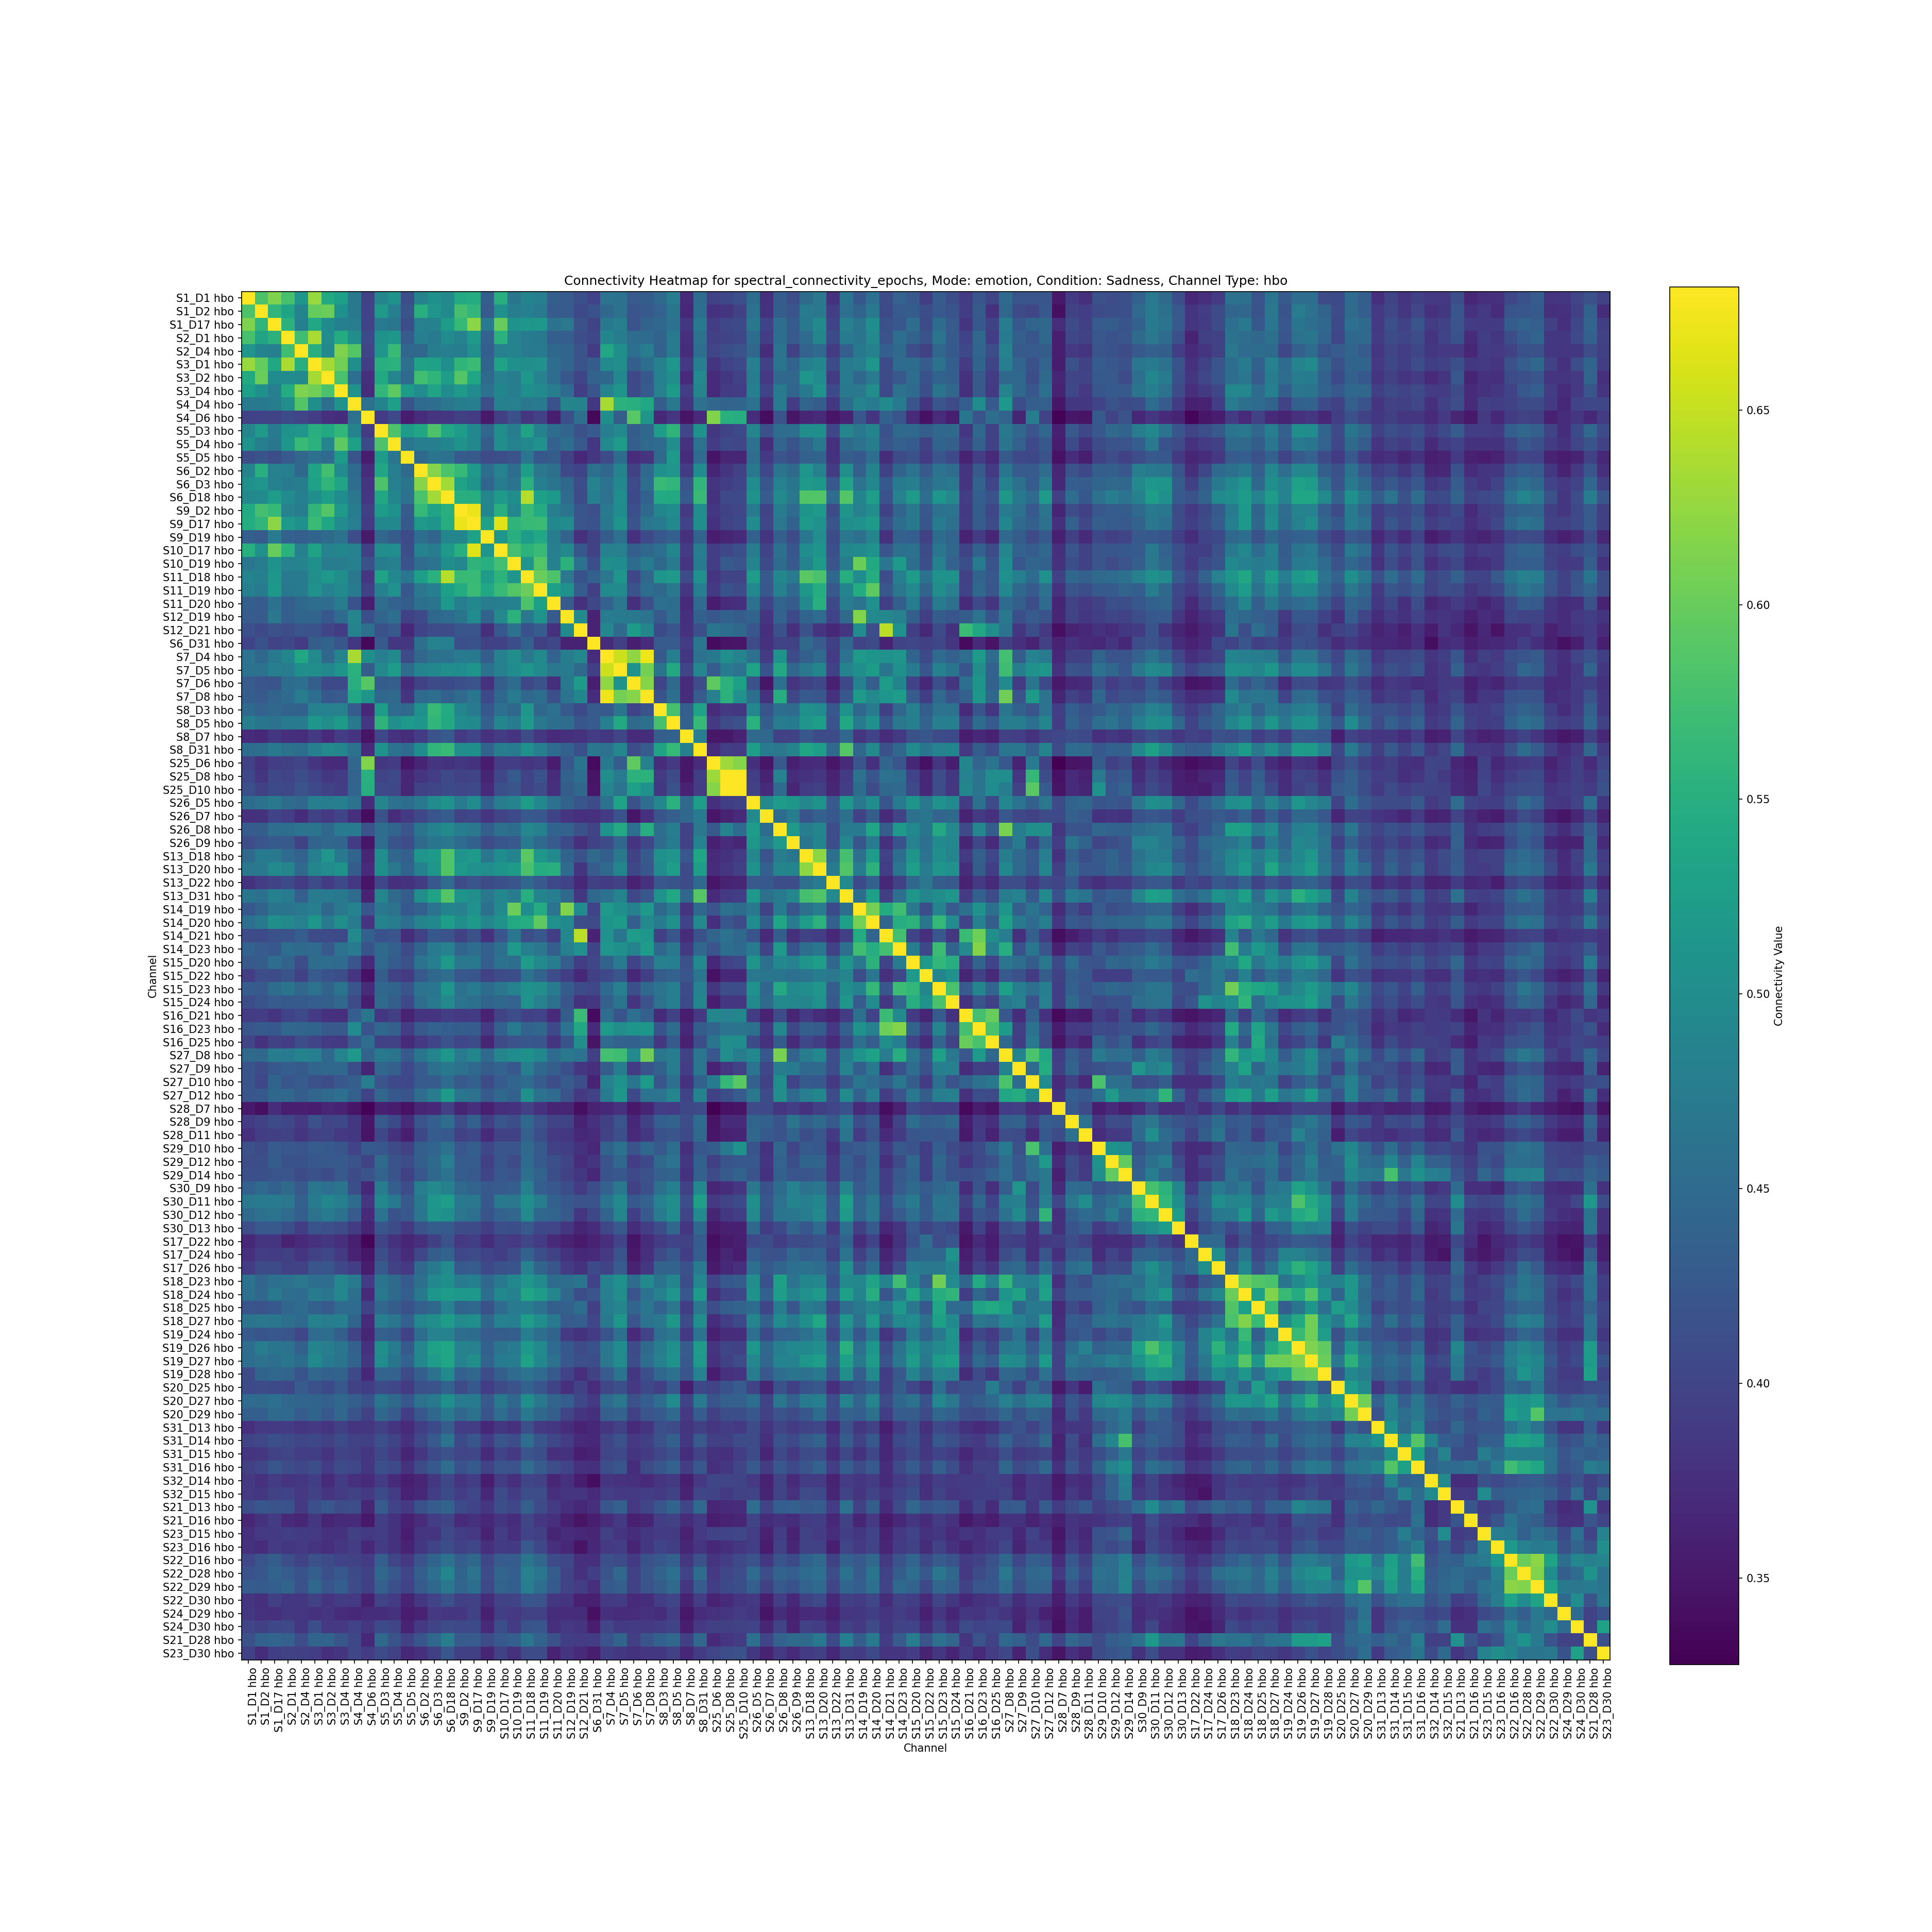
\includegraphics[width=\textwidth]{C:/Users/super/OneDrive - Ontario Tech University/fNIRS_Emotions/plots/connectivity/chord_plots/conditions/emotion_Sadness_con.png}
    \end{minipage}
    \begin{minipage}[t]{0.45\textwidth}
        \vspace{-\baselineskip}
        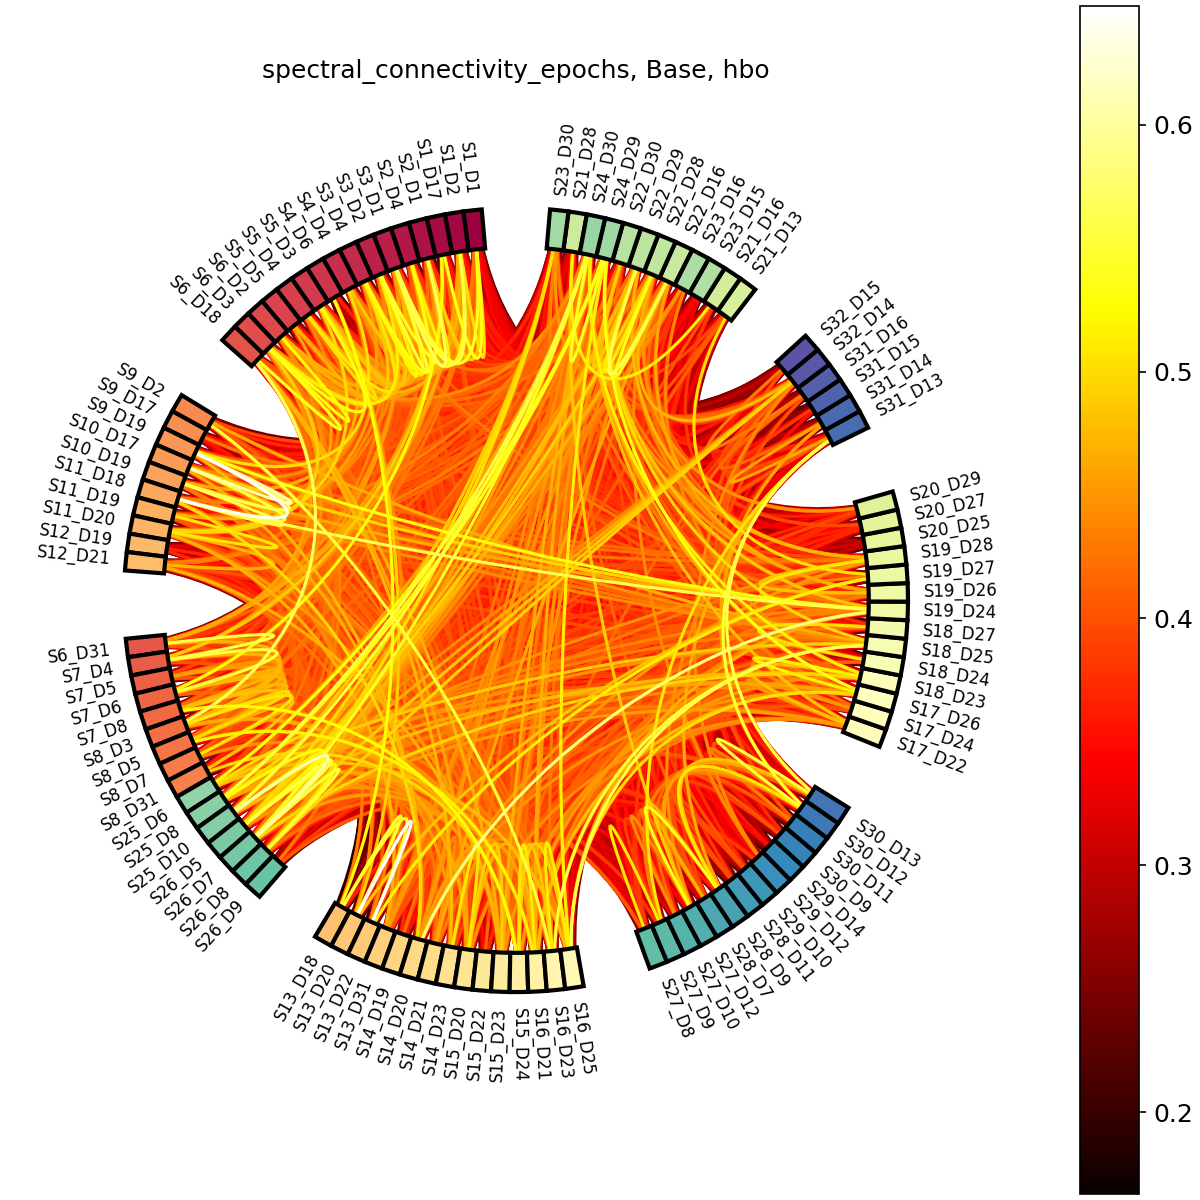
\includegraphics[width=\textwidth]{C:/Users/super/OneDrive - Ontario Tech University/fNIRS_Emotions/plots/connectivity/chord_plots/conditions/face_type_Base_con.png}
    \end{minipage}
    \begin{figure}
        \caption{Chord plot of connectivity between channels for sadness (left) and baseline (right) conditions. Brighter lines represent higher connectivity strength.}
        \begin{itemize}
            \item Connections across the middle of the plot indicate connectivity across far apart regions of the brain.
        \end{itemize}
    \end{figure}
\end{frame}

% display C:\Users\super\OneDrive - Ontario Tech University\fNIRS_Emotions\plots\connectivity\chord_plots\group_level_t_tests\face_type_Real_Virt_p_values.png
% display C:\Users\super\OneDrive - Ontario Tech University\fNIRS_Emotions\plots\connectivity\chord_plots\group_level_t_tests_neutral\emotion_Joy_Neutral_p_values.png
% display these two side by side
\begin{frame}
    \frametitle{Connectivity Group Level T-Tests Chord Plots}
    \begin{minipage}[t]{0.45\textwidth}
        \vspace{-\baselineskip}
        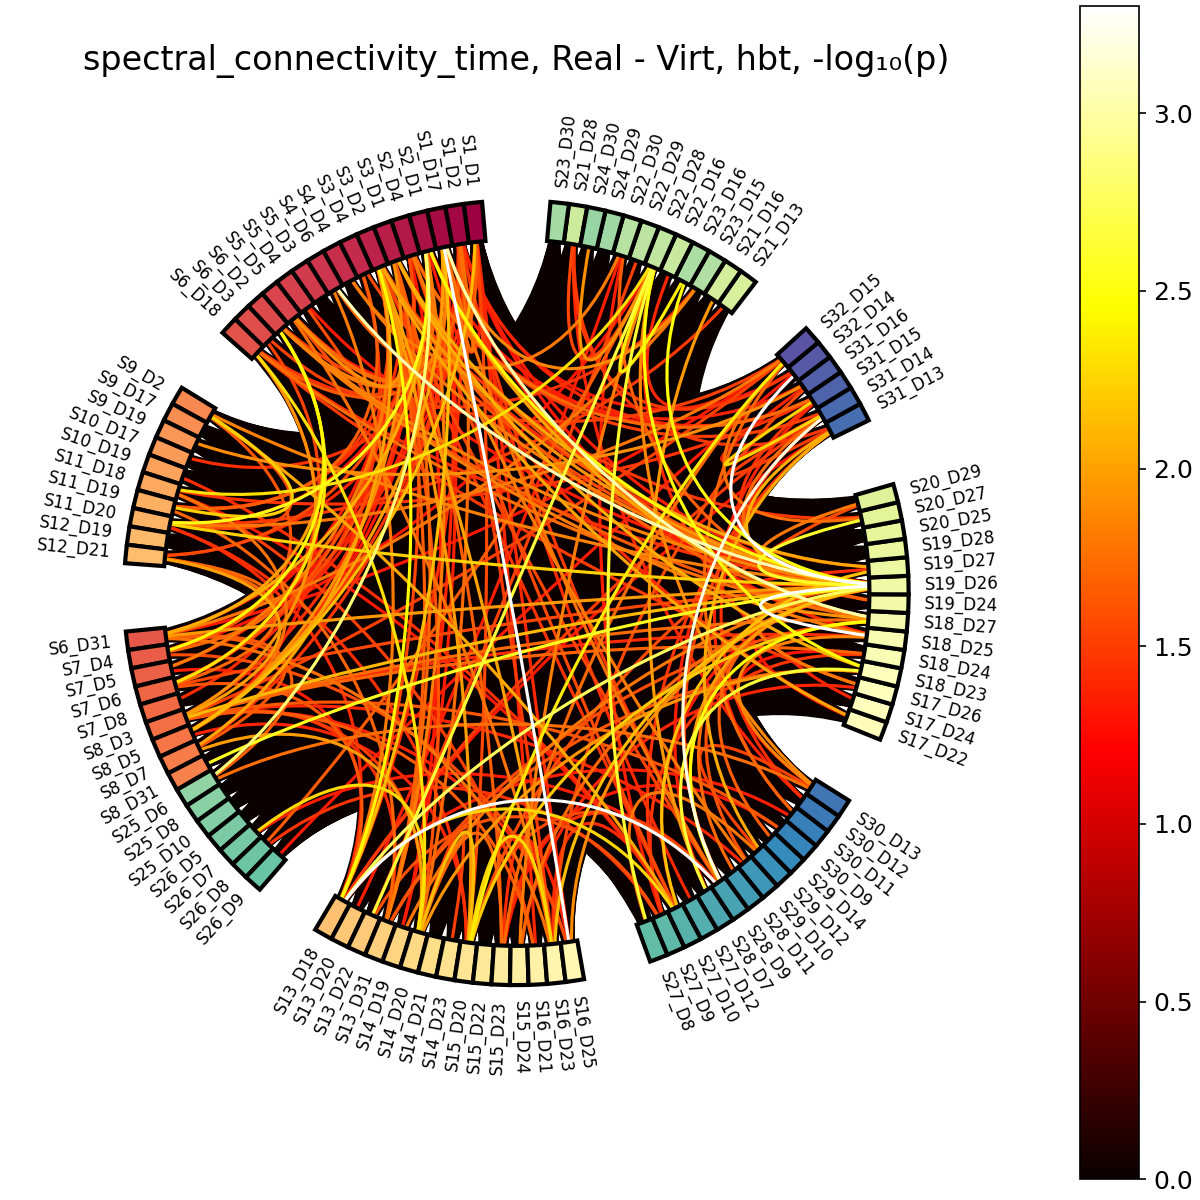
\includegraphics[width=\textwidth]{C:/Users/super/OneDrive - Ontario Tech University/fNIRS_Emotions/plots/connectivity/chord_plots/group_level_t_tests/face_type_Real_Virt_p_values.png}
    \end{minipage}
    \begin{minipage}[t]{0.45\textwidth}
        \vspace{-\baselineskip}
        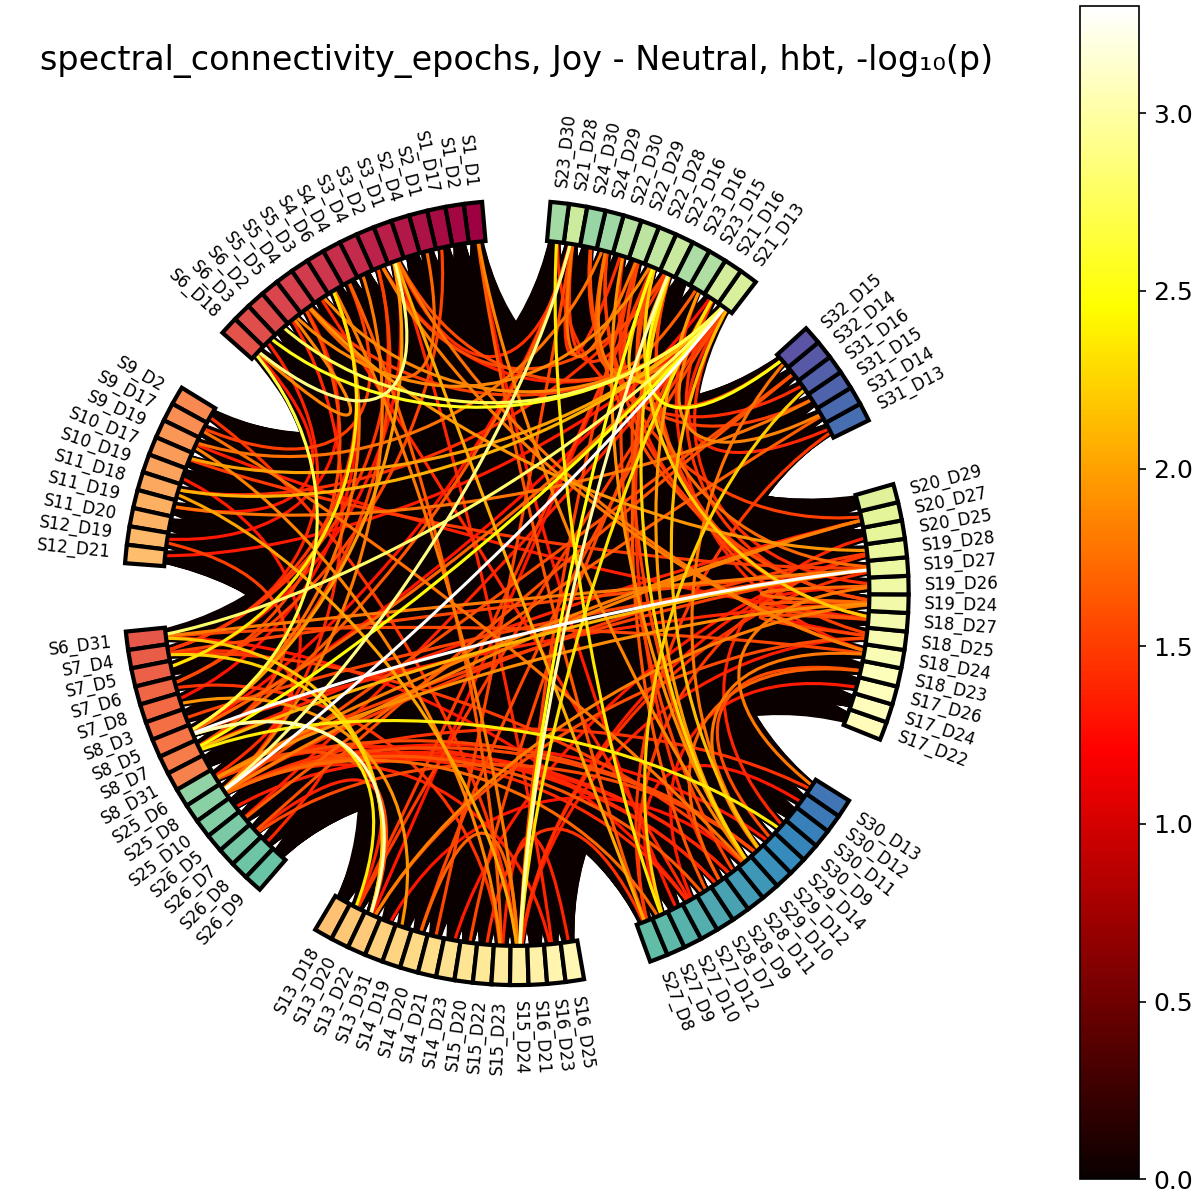
\includegraphics[width=\textwidth]{C:/Users/super/OneDrive - Ontario Tech University/fNIRS_Emotions/plots/connectivity/chord_plots/group_level_t_tests_neutral/emotion_Joy_Neutral_p_values.png}
    \end{minipage}
    \begin{figure}
        \caption{Paired t-tests were conducted on Fisher $z$-transformed connectivity matrices (reshaped from averaged channel-specific data) for each unique pair of conditions (i.e. Real vs. Virtual (left) and Joy vs. Neutral (right)).
        $p$-values were computed for each lower-triangular matrix element across participants and subsequently corrected for multiple comparisons using False Discovery Rate (FDR) correction.}
    \end{figure}
\end{frame}

% display C:\Users\super\OneDrive - Ontario Tech University\fNIRS_Emotions\plots\models\model_scores.png
\begin{frame}
    \frametitle{Decoding Analysis}
    \begin{figure}
        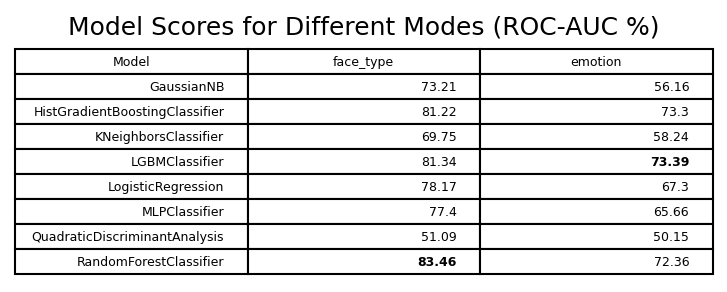
\includegraphics[width=1\textwidth]{C:/Users/super/OneDrive - Ontario Tech University/fNIRS_Emotions/plots/models/model_scores.png}
        \caption{Spatio-temporal classification performance of multiple machine learning models across conditions. For each model, recordings were preprocessed via scaling and vectorization. The average ROC-AUC scores were computed using five-fold cross-validation over all recordings. }
    \end{figure}
\end{frame}

\end{document}